\section{CBP response calibration with a solar cell}
\label{sec:rcbp}

\subsection{Preparatory settings}

Before illuminating the solar cell with the CBP, several actions have to be taken to maximise the quality of the data sets:
\begin{itemize}
\item place the pinholes at the focus of the CBP telescope
\item tune the telescope iris
\item align the CBP and the solar cell in position and angle
\item mask every ambient light
\item spectrograph calibration
\item \todo{think a lot about what we forgot}
\end{itemize}


\subsubsection{Iris}

\todo{Marc}

\subsubsection{Focussing}

\todo{Marc}


The CBP was aligned with the StarDICE telescope to improve the focus. The
StarDICE camera was set close to infinity with no filter (focus encoder:
8mm). The smallest pinhole (\SI{75}{\um}). Elana adjusted the CBP focus to get the smallest extension of the pinhole
image. A slight offset was then added to account for the small change in focus
introduced by tightening the locking screws. Here is a confirming image taken
just after.

The focus was to check to resist slot changes and even complete removal and
reinstallation of the pinhole.

For the record, mount coordinates to get CBP and telescope aligned were
$[13.199987411499023, 1.4999985694885254]$



\subsubsection{Alignment of the CBP}

To measure the CBP response, we must ensure that we aim toward the solar cell. For that, we studied the signal collected in the solar cell $\Qsolarmes$ with respect to the CBP mount coordinates in azimuth and altitude. We defined the position at which we park the CBP mount when no measurement is taken at $(\mathrm{alt} = \SI{0}{\degree}, \mathrm{az} = \SI{0}{\degree})$, and the coordinates in the figure \ref{fig:cross_sc} are relative to this origin. With this figure, we can estimate the coordinates at which $\Qsolarmes$ is maximum, corresponding to the solar cell coordinates in the CBP mount frame of reference. We set the solar cell coordinates at $(\mathrm{alt} = \SI{6}{\degree}, \mathrm{az} = \SI{10}{\degree})$. These coordinates correspond to the point aimed by the CBP optics for any further solar cell analysis in this paper.

\begin{figure}[h]
    \centering
    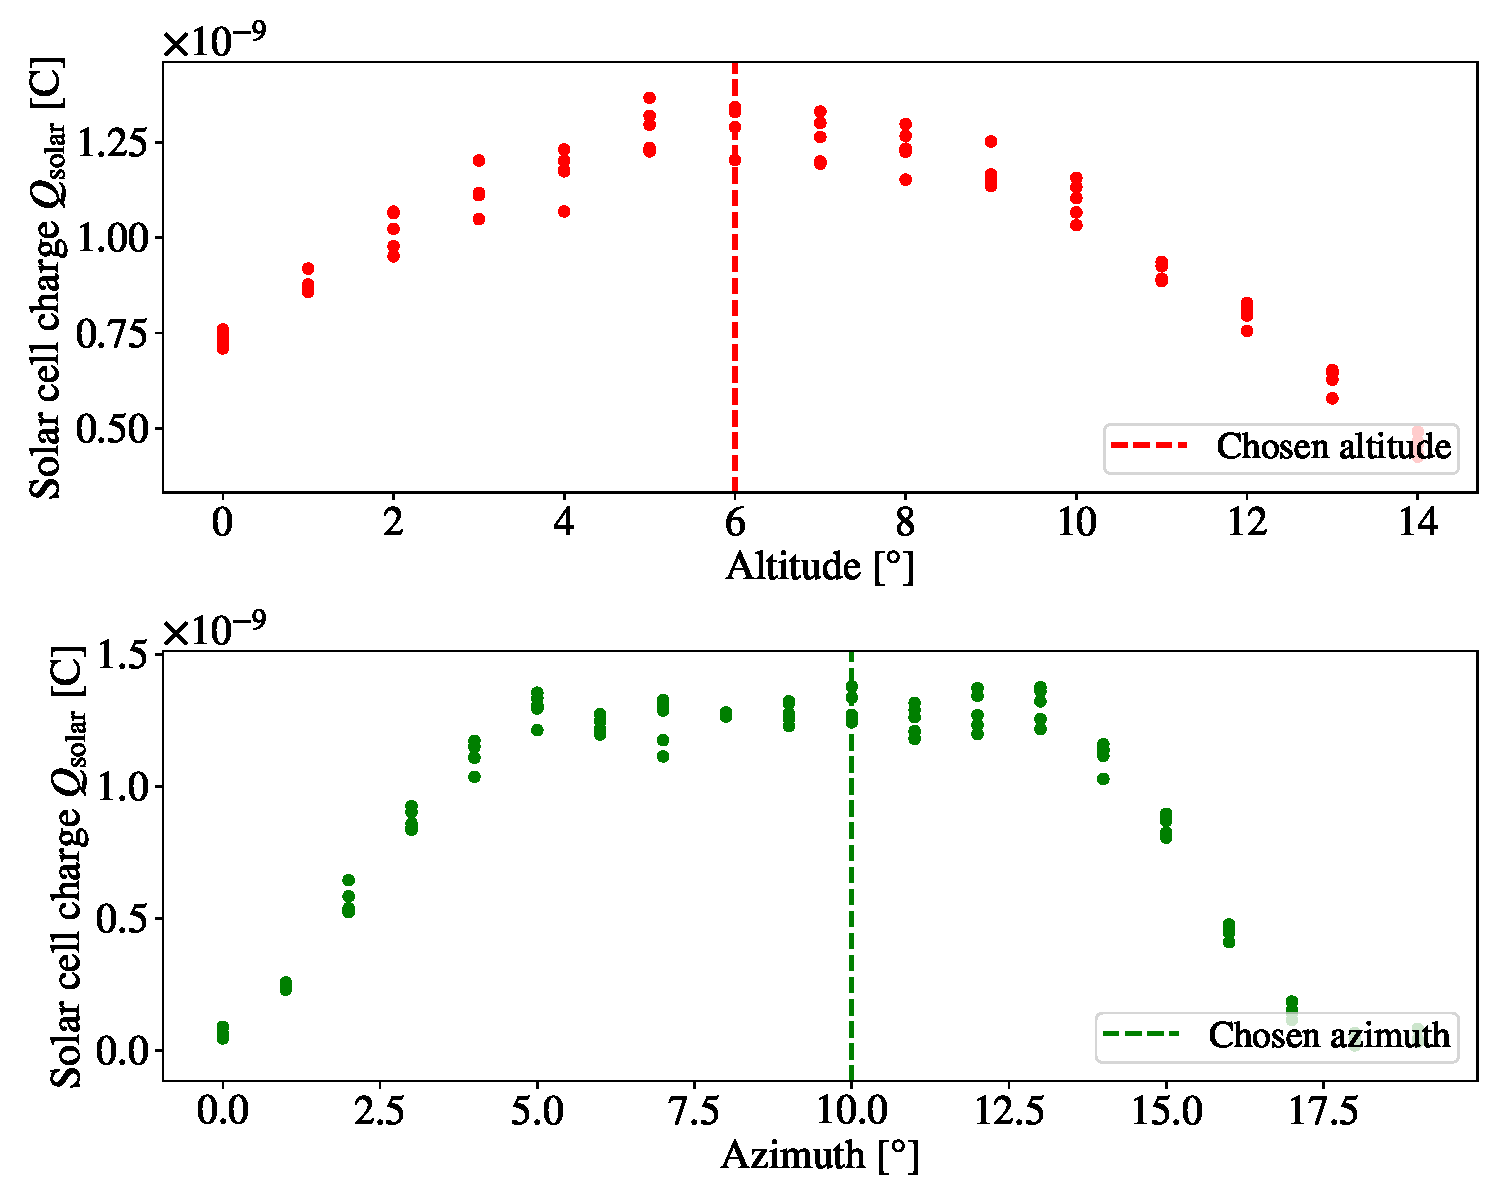
\includegraphics[width=\columnwidth]{fig/cross_solarcell.pdf}
    \caption{Evolution of the solar cell charge $\Qsolarmes$ with respect to the CBP mount coordinates. Left: evolution with respect to the altitude coordinate. Right: evolution with respect to the azimuth coordinate.}
    \label{fig:cross_sc}
    %/stardice/analysis/cbp_paper/golden_sample_analysis/dr2/cross_solarcell.ipynb
\end{figure}

\subsubsection{Ambient light}

Depending on their direction, ambient light can contaminate sensitive devices in the lab room. We masked all diodes from computers or electronic devices.

\subsubsection{Spectrograph error model estimation and wavelength calibration}

The spectrograph was characterised by taking a series of dark exposures with four different exposure times (the same used in the CBP response measurement) to evaluate its gain and readout noise. The goal is to build an error model for the spectrograph.

For each exposure time, a master dark is constructed, averaging all the spectra. Then, for each spectrograph pixel, we fitted a line through the master dark values as a function of the exposure times. The intercept gave the sensor bias value for each pixel, and a master bias $B(\lambda_p)$ is assembled from the intercept values, with $\lambda_p$ the raw spectrograph wavelength value before any calibration associated with each sensor pixel $p$. 

The master bias was subtracted from all dark exposures. From those data, we measured the readout noise and sensor gain. Let's call $D(\lambda_p)$ the dark exposure minus the master bias value for pixel $p$. For each exposure time, the variance $\sigma_p^2$ and average $\bar{D}(\lambda_p)$ of each $D(\lambda_p)$ pixel were computed. The variance evolution with the average is well described by a second-order polynomial function, parameterised as follows:
\begin{equation}\label{eq:spectro_error_model}
\sigma^2_p =\sigma_{ro}^2 +  \bar{D}(\lambda_p)/G + \sigma_G^2 \bar{D}^2(\lambda_p)
\end{equation}
with $\sigma_{ro}$ the readout noise, $G$ the sensor gain and $\sigma_G$ a statistical noise on the gain itself. The fit of this model to data led to the following values (Figure~\ref{fig:spectro_ptc}):
\begin{align}
    \sigma_{ro} &= 1.26\ \mathrm{ADU}, \\
    G & = 25.8\ e^-/\mathrm{ADU} ,\\
    \sigma_G & = 0.7\%.
\end{align}
The first two values are compatible with the CCD specifications given by the spectrograph vendor. 

%spectrograph_dark_and_bias.py
\begin{figure}[!h]
\centering
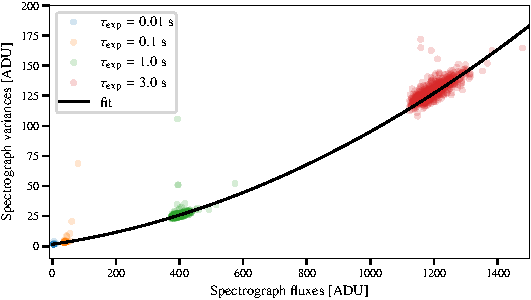
\includegraphics[width=\columnwidth]{spectro_ptc}
\caption{Spectrograph photon transfer curve to estimate gain and read-out noise. Pixel variance from dark spectra is represented versus their averages for four different exposure times $\tau_{\mathrm{exp}}$.}\label{fig:spectro_ptc}
\end{figure}


We calibrated the spectrograph according to the manufacturer's specifications before and after the main data acquisition run to measure the CBP and \SD responses. Light from a Hg-Ar lamp was injected into the integrating sphere to illuminate the spectrograph sensor. The master bias $B(\lambda_p)$ was subtracted from all spectra. The latter were stacked, and the spectrograph error model from equation~\ref{eq:spectro_error_model} was used to get a first estimate of the intensity uncertainties. The emission lines were fitted on the stacked spectrum using Gaussian profiles plus a polynomial background. Let's call $\lambda_g$ the line centroid fitted by this Gaussian profile. The fit is unweighted to avoid any dependence of $\lambda_g$ with the line flux and checked it was the case, but a statistical uncertainty $\sigma_\lambda^{\rm noise}$ is still estimated for $\lambda_g$ as 
\begin{equation}\label{eq:sigma_lambda_stat}
    \sigma_\lambda^{\rm noise}= \dfrac{1}{\sum_k F_k} \sqrt{\sum_p \left(\lambda_p - \lambda_g\right)^2 \sigma_p^2}
\end{equation}
with $F_k$ the flux in pixel $k$ after master bias subtraction. The sums are performed over a window of size $\pm 3 \sigma_g$ around $\lambda_g$ where $\sigma_g$ is the fitted line Gaussian profile RMS. Equation~\ref{eq:sigma_lambda_stat} corresponds to the propagation uncertainty formula for the average wavelength weighted by flux $F_p$ in a $\pm 3 \sigma_g$  window around $\lambda_g$. Doing so, we considered the shot-noise without biasing our $\lambda_g$ fit.

To transform raw sensor wavelengths $\lambda_p$ into calibrated wavelengths $\lambda_c$, we fitted a third-order polynomial function as requested by the manufacturer to minimise the distance to Hg-Ar tabulated values $\lambda_t$. In doing so, we minimised the following function 
\begin{equation}
    \chi_\lambda^2(a_3, a_2, a_1, a_0) = \sum_{\text{lines}} \left(\lambda_t-a_3 \lambda_g^3 - a_2 \lambda_g^2-a_1 \lambda_g -a_0\right)^2
\end{equation}
over the four polynomial coefficients $a_3, a_2, a_1$ and $a_0$. The sum is performed over lines with high significance (signal-to-noise ratio above 20), and known doublet lines were excluded. The minimisation leads to the four best-fit parameters $\hat a_i$ associated with their covariance matrix. 
As the initial Gaussian fit was unweighted, the covariance matrix is then re-scaled with a global factor to get a final reduced $\chi_\lambda^2$ of one: let's call it $\mathbf{C}_\lambda$. 
Finally, detected line centroids $\lambda_g$ are transformed into calibrated wavelengths $\lambda_c$ using the third order polynomial function $c(\lambda_g)$ with the four best fit parameters:  
\begin{equation}
    \lambda_c \equiv c(\lambda_g) \equiv \hat a_3 \lambda_g^3 + \hat a_2 \lambda_g^2+\hat a_1 \lambda_g +\hat a_0
\end{equation}
and the $\sigma_\lambda^{\rm cal}$ calibration uncertainties are
\begin{equation}
    \sigma_\lambda^{\rm cal} = \left(\vec J_c^T \mathbf{C}_\lambda \vec J_c\right)^{1/2},\quad \vec J_c = \left(\lambda_g^3, \lambda_g^2, \lambda_g, 1\right).
\end{equation}

In Figure~\ref{fig:spectro_calib_syst}, we plot the residuals of the fit $c(\lambda_g)-\lambda_t$ in the upper panel, showing the agreement between the re-scaled data uncertainties and the uncertainties propagated to the third order polynomial function $c(\lambda_g)$ using $\mathbf{C}_\lambda$. In the lower panel, the spectrograph calibration systematic uncertainties $\sigma_\lambda^{\rm cal}$ are emphasised: they are lower than $\SI{0.1}{\nm}$ in the entire wavelength range, even lower than \SI{0.025}{\nm} in the visible spectrum.

%spectrograph_calibration.py
\begin{figure}[!h]
\centering
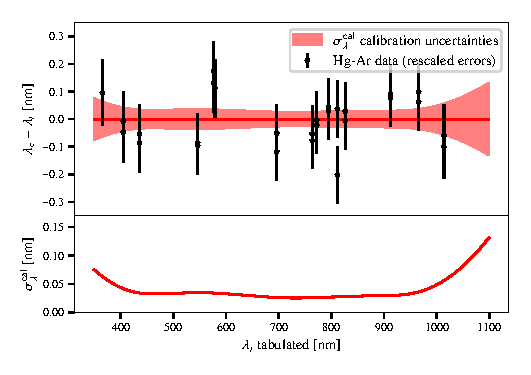
\includegraphics[width=\columnwidth]{spectrograph_calibration_syst}
\caption{Spectrograph calibration plot. Top: difference between the tabulated Hg-Ar emission line wavelengths $\lambda_t$ and the wavelengths computed using the spectrograph calibration function $c(\lambda_g)$. Data taken before and after the data acquisition campaign are superimposed. Their uncertainties were re-scaled with a common factor to get a final reduced $\chi^2$ of one. The red band represents the systematic uncertainty band from the $c(\lambda_g)$ fit on data with the uncertainty rescaling. Bottom: emphasis on the systematic uncertainties of the spectrograph calibration procedure.}\label{fig:spectro_calib_syst}
\end{figure}

During the data acquisition campaign, we did not unplug and plug again the optical fibre going from the integrating sphere to the spectrograph. Such an action on the spectrograph side could have changed the wavelength calibration in principle, even if beforehand, we checked the fibre placement in the spectrograph was very reproducible and did not change the wavelength scale.
 
\subsection{Data set description}
\label{sec:cbp_datadesc}

\begin{figure*}[!h]
\centering
%cbp_paper_plots
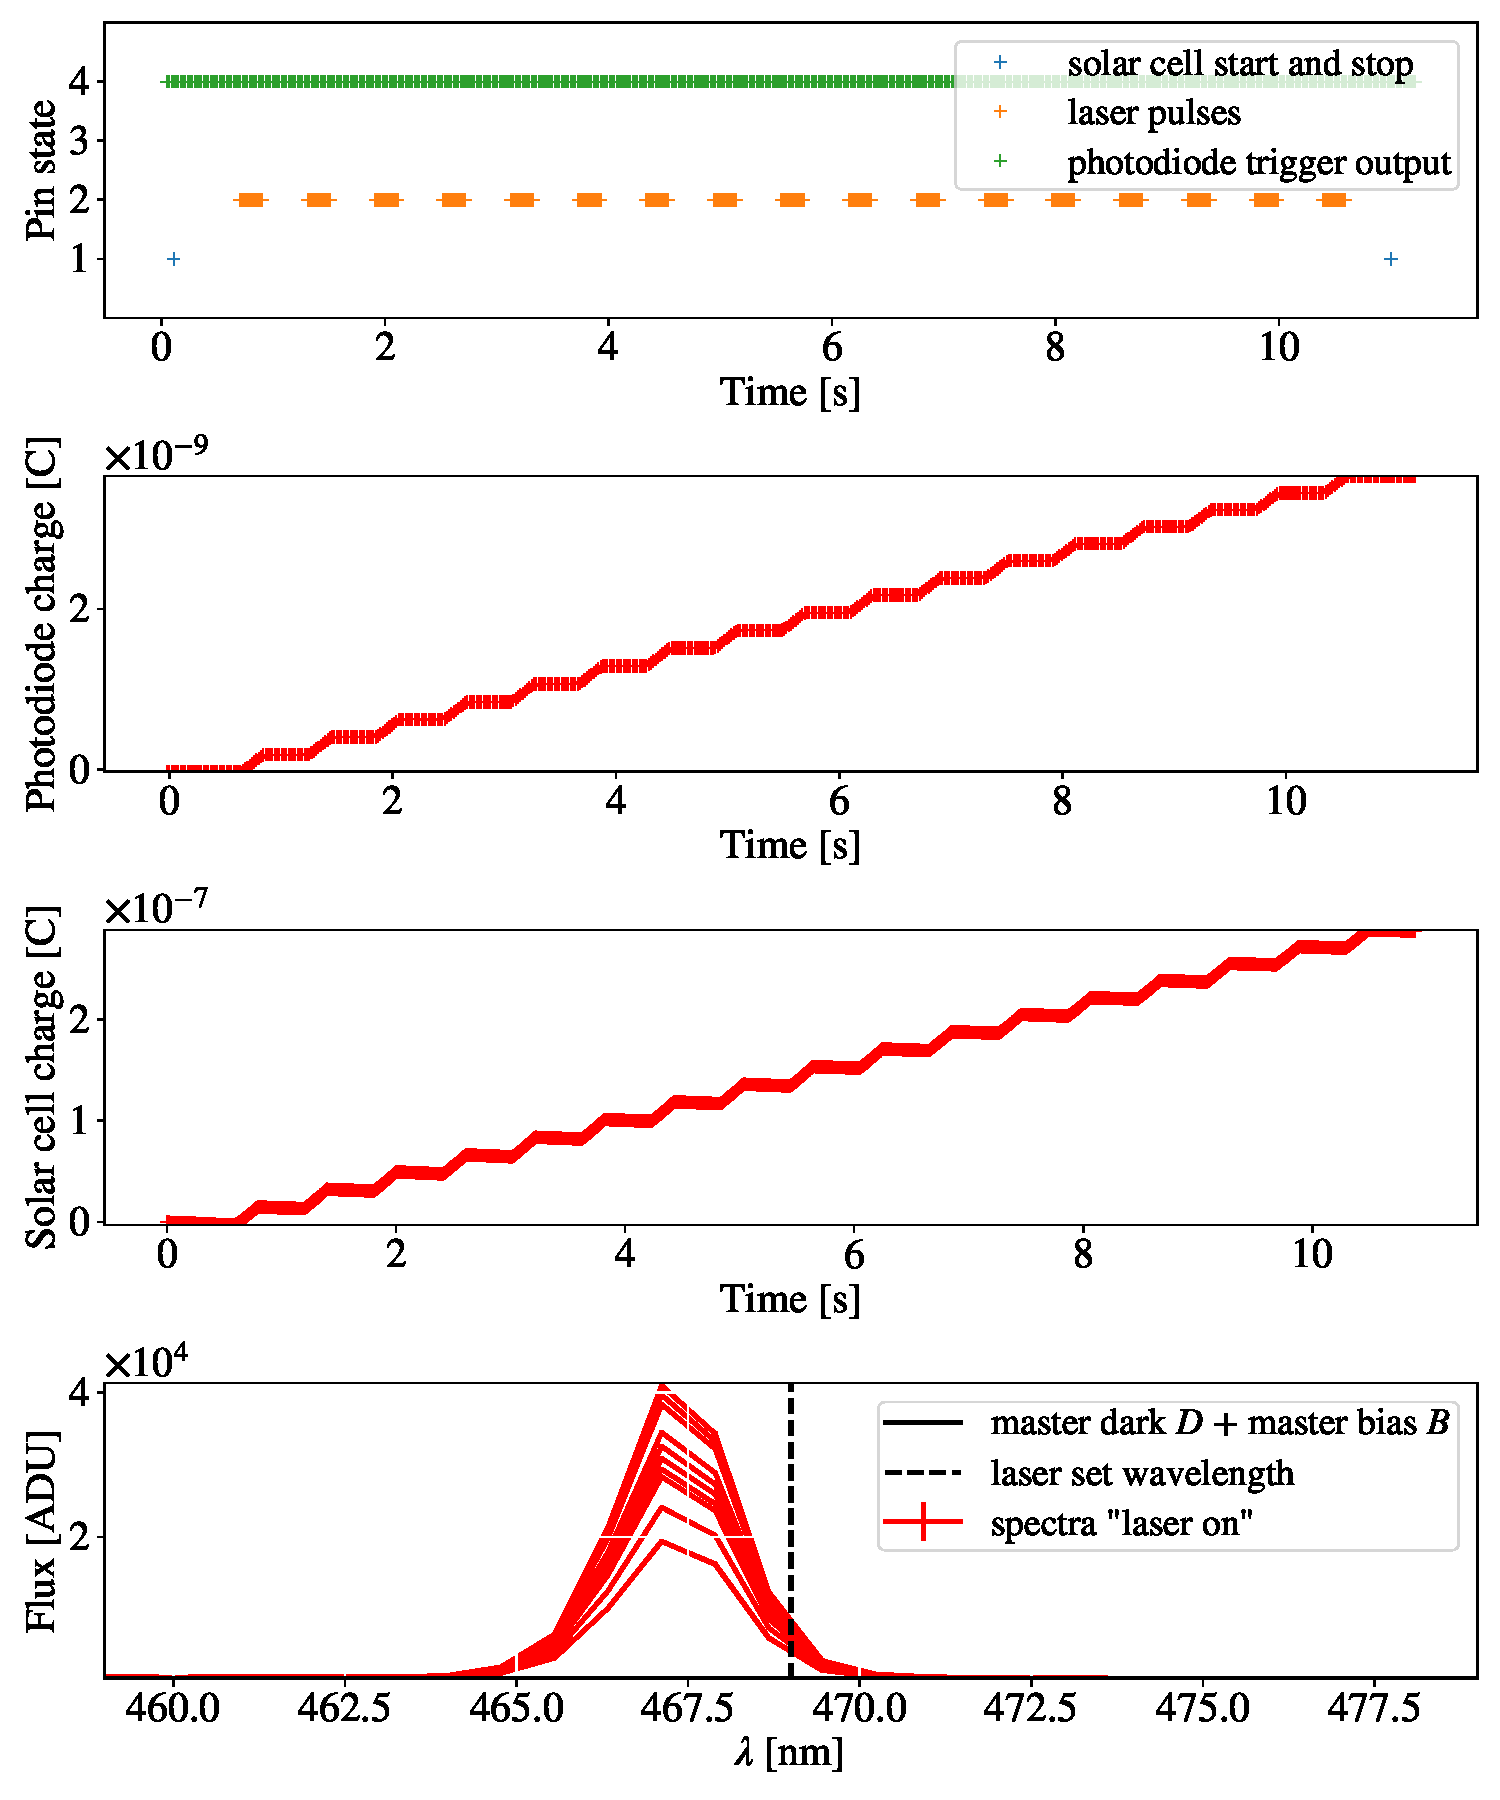
\includegraphics[width=\columnwidth]{sc_dataset_469}
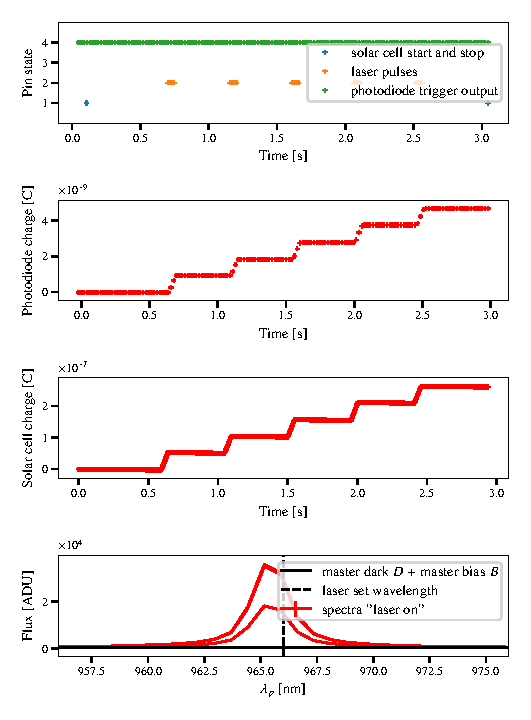
\includegraphics[width=\columnwidth]{sc_dataset_966}
\caption{Data set examples. From top to bottom: typical data sets for digital analyser (pin state 4 is the Keithley output, pin state 2 the laser trigger output, pin state 1 the Keysight start and end time acquisition time stamps), charges in the photodiode, charges in the solar cell, flux in the spectrograph. Left: typical data set at \SI{469}{\nm}. Right: typical data set at \SI{966}{\nm}.}\label{fig:sc_dataset_examples}
\end{figure*}

A typical dataset to measure the CBP response is the emission of laser bursts in the solar cell at a given wavelength. Charges in the photodiode and solar cell are recorded jointly, along with the flux in the spectrograph and the time stamps in the digital analyser (see examples in Figure~\ref{fig:sc_dataset_examples}).

The laser emits pulses at a fixed rate of \SI{1}{\kilo\hertz}, with a power that highly depends on the wavelength. To ensure that all instruments work in their linear regime, without saturations, and control the dark current, we decided to shoot light in the solar cell in bursts of pulses, separated by dark times at least as long as the burst length. The number of pulses was set to maintain a relatively constant total accumulated charge in the monitoring photodiode, which is the common instrument between the CBP and \SD response measurements and the one receiving the maximum power in the system (Figure~\ref{fig:npulses}). Therefore, we expect to minimise eventual non-linear effects in the instrumental chain. The CBP system's linearity is checked by varying the laser power in Section~\ref{sec:sc_linearity}. However, we know we have a $1/f$ noise in the solar cell instrumental chain. To limit the amplitude of these random fluctuations during the burst, we set the maximum number of pulses to 200 (so \SI{200}{\ms}). If more pulses were requested to maintain the signal level in the photodiode, we compensated with a higher number of bursts.

We used the \SI{5}{\mm} pinhole with the largest laser power mode to get the highest signal-to-noise ratio in the solar cell and the \SD telescope. The solar cell accumulates around \SI{4}{\nano\coulomb} in a burst, with no change of Keysight range. % The Keysight accuracy in this regime is \todo{to check}. 
During a solar cell measurement run, the laser wavelengths range between \SI{350}{\nano\meter} and \SI{1100}{\nano\meter} included with steps of \SI{1}{\nm}, but are randomly chosen to avoid that long-range $ 1/f$ mode in the solar cell dark current correlates neighboured data points of the CBP response. Several runs were accumulated to enhance the signal-to-noise ratio. In particular, five runs were recorded just before the \SD telescope measurement, and five new runs were launched just after.

Runs with different settings have been conducted to estimate systematic uncertainties. We varied the laser global power (QSW) to assess the linearity of the instrumental light and check the ambient light additive contamination. We varied the solar cell distance to estimate the output CBP scattered light.

%cbp_paper_plots.py
\begin{figure}[!h]
\centering
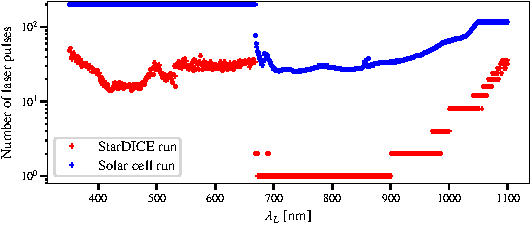
\includegraphics[width=\columnwidth]{npulses}
\caption{Number of laser pulses per burst used for solar cell and StarDice runs.}\label{fig:npulses}
\end{figure}


\subsection{Data reduction}

\todo{check that time stamps are explicitly described for all data sets}

In one data set, we accumulated several laser bursts, and a per-burst analysis was conducted to be able to remove outliers more easily. All bursts are combined only at the end of the analysis to get the CBP and StarDice responses.

\subsubsection{Photodiode data reduction overview}
\label{sec:pd_reduction}

Photodiode data are charge time series with stair-case shape. Each step is a laser burst, and the step height roughly gives the charge $\Qphotmes$ accumulated during a laser burst (see Figures~\ref{fig:sc_dataset_examples} and~\ref{fig:pd_reduc}). The length of the charge rise is the laser burst duration $\tau_b$ while flat sequences are dark times. For the photodiode, the time stamps come directly from the digital analyser clock, with a sampling at \SI{50}{\hertz}. The digital analyser clock also provides the time stamps of the laser pulses. 

For each burst, we fit straight lines in the charge sequence during the dark times before and after a laser burst, removing the closest points to the burst. We call $t_1$ and $t_2$ the time stamps of the beginning and ending of the laser burst, respectively, given by the laser trigger output itself.%\footnote{Technically, the laser time stamps provide the beginning of the pulse, so we add \SI{1}{\ms} to the last trigger time stamps from the laser to account for the pulse duration.}. 
The accumulated charge $\Qphotmes$ during a burst is then
\begin{align}
q_{\rm phot}^{\rm dark}(t)  = & a_{\rm phot} t + b_{\rm phot} \\
\Qphotmes  = & q_{\rm phot,2}^{\rm dark}(t_2) - q_{\rm phot,1}^{\rm dark}(t_1)\\ & - \frac{1}{2} \left[ q_{\rm phot,1}^{\rm dark}(t_2) -  q_{\rm phot,1}^{\rm dark}(t_1) + q_{\rm phot,2}^{\rm dark}(t_2) - q_{\rm phot,2}^{\rm dark}(t_1)  \right]   \notag 
\end{align}
where $q_{\rm phot,j}^{\rm dark}(t_i)$ is the line fit of the dark part $j$ ($j=1$ before the burst, $j=2$ after) evaluated at time $t_i$. Doing so, the subtraction $q_{\rm phot,2}^{\rm dark}(t_2) - q_{\rm phot,1}^{\rm dark}(t_1)$ gives the raw height of the burst step in the charge sequence\footnote{Moreover, doing the subtraction removes systematics inaccuracy coming from the Keithley electrometer.} while the terms in brackets remove the averaged contribution of the dark current using both dark times before and after the burst. Note that we do not model anything during the burst time, as the laser power stability does not guarantee that this can be modelled with a simple mathematical function. The only model assumption is that dark sequences are modelled with straight lines.

The fit of the two parameters $a_{\rm phot}$ and $b_{\rm phot}$ of each $q_{\rm phot,j}^{\rm dark}(t)$ line models is performed via a standard $\chi^2$ minimisation, using the \texttt{curve\_fit} method from python library \texttt{scipy}. Uncertainties on the data points, equally weighted, are tuned so that the final reduced $\chi^2$ is one. Doing so, we assume that the fit residuals are only due to Gaussian instrumental noise, as justified by Figure~\ref{fig:pd_reduc}. The analysis of the residuals also confirms our choice to use order 1 polynomial functions to model the dark sequences.



%cbp_paper_plots.py
\begin{figure}[!h]
\centering
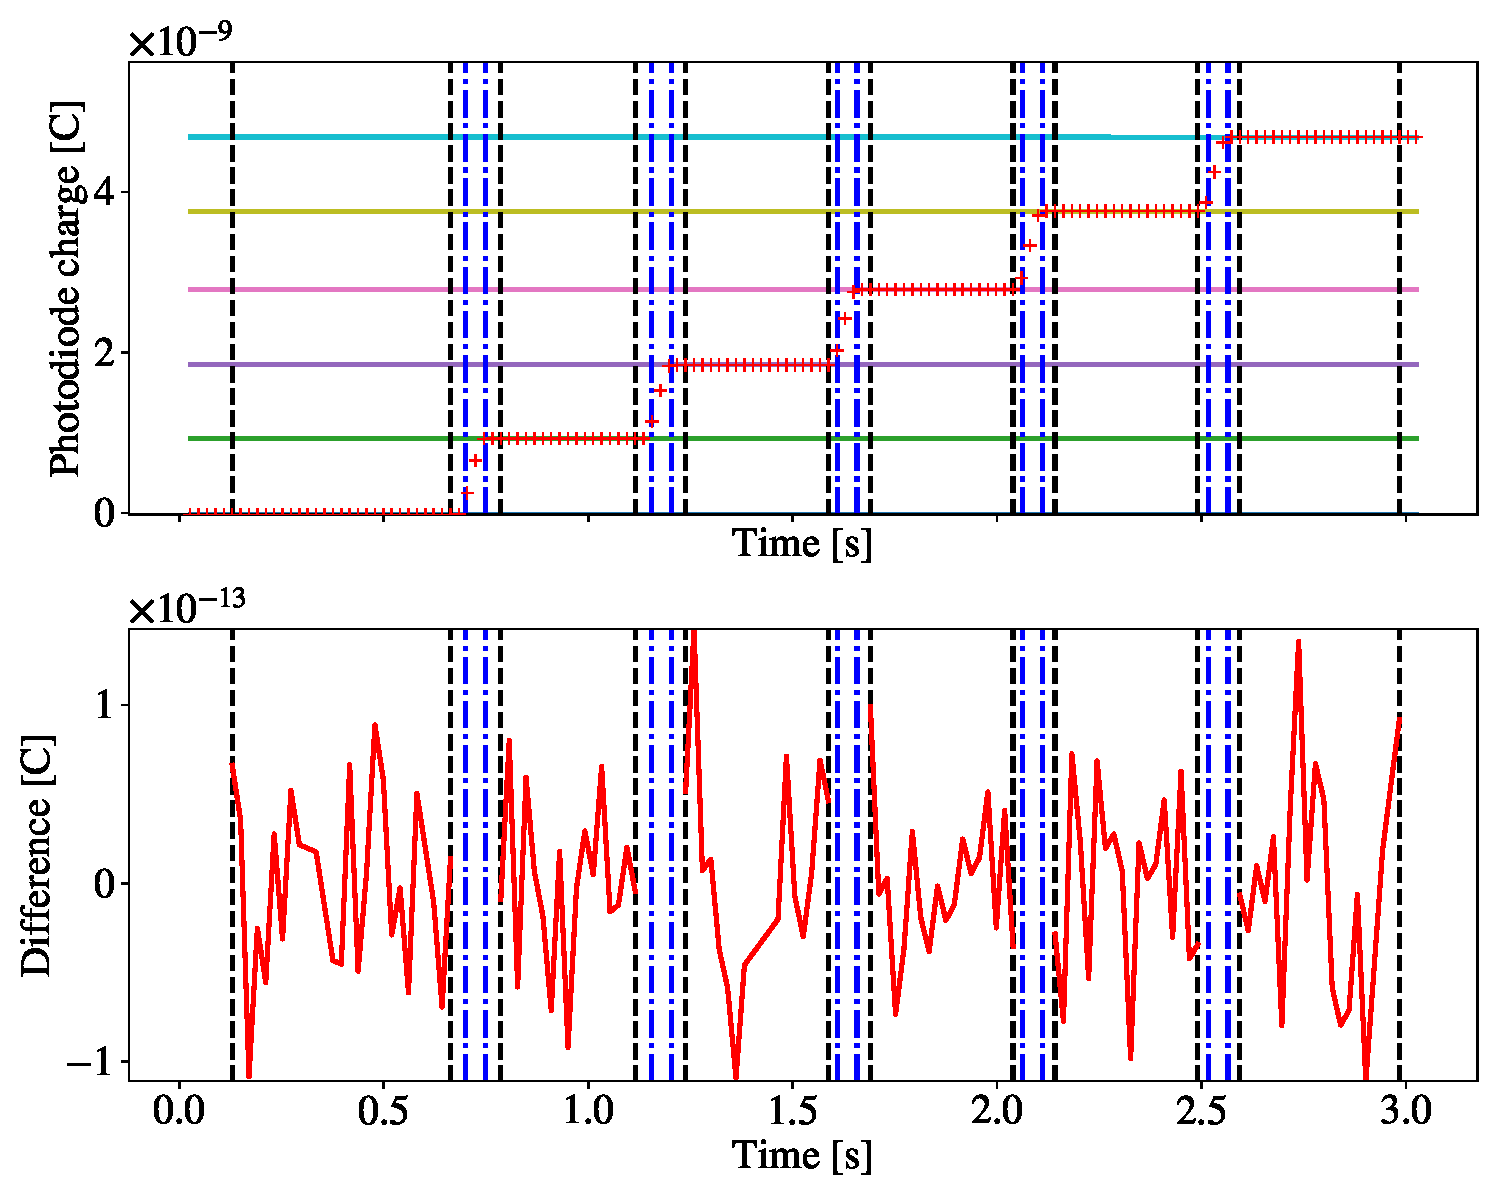
\includegraphics[width=\columnwidth]{pd_reduc_966}
\caption{Photodiode charge sequence reduction process at wavelength $\lambda_L=\SI{469}{\nm}$. Vertical blue lines indicate the laser starts and stops, while black lines flank the dark sequences. Coloured horizontal lines are fitted during dark times. The top panel shows the raw charges acquired with the photodiode, while the bottom panel shows the residuals of the linear fits during dark times.}\label{fig:pd_reduc}
\end{figure}

Covariance matrix uncertainties from all linear model parameters are then propagated to compute the statistical uncertainty $\Sphotstat$ of $\Qphotmes$ per burst. They are typically of the order of the residual RMS, around \SI{5e-5}{\nano\coulomb} (Figure~\ref{fig:pd_reduc}), more than three orders of magnitude below the typical $\Qphotmes$ values. We tested the fitting procedure on pure dark sequences and found an unbiased null measurement $\Qphot^{\rm dark}$ with a pull distribution of RMS $\;\approx 1$ whatever the burst duration $\tau_b$: computed statistical uncertainties $\Sphotstat$ nicely covers the data Gaussian noise (Figure~\ref{fig:charge_pull}).

%stardice_analysis/keithley_dark_and_bias.py
\begin{figure}[!h]
\centering
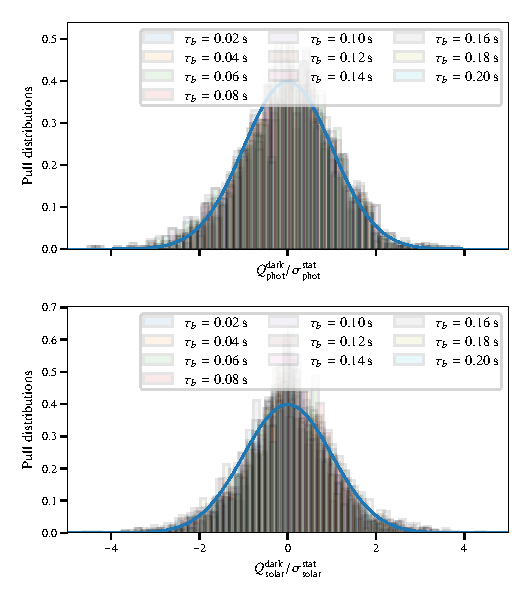
\includegraphics[width=\columnwidth]{pd_sc_stat_pull}
\caption{Top: pull distributions for photodiode charge measurements during pure dark time series $\Qphot^{\rm dark} / \Sphotstat$, with different burst durations $\tau_b$. Cyan curve represents a Gaussian distribution of mean 0 and RMS 1. Bottom: same but for the solar cell case $\Qsolar^{\rm dark} / \Ssolarstat$.}\label{fig:charge_pull}
\end{figure}



\subsubsection{Solar cell data reduction overview}
\label{sec:solar_reduction}

Solar cell charge time series are very similar to photodiode time series (see Figures~\ref{fig:sc_dataset_examples} and~\ref{fig:sc_reduc}). However, they are affected by two supplementary contributions as seen in the noise power spectrum: a random $1/f$ noise and power line harmonics mainly at \SI{50}{\hertz} and \SI{100}{\hertz} (Figure~\ref{fig:darkcurrentspectrum}). Timestamps come directly from the Keysight electrometer. However, as this device sends triggers at the start and end of the acquisition, the electrometer clock is re-scaled using the digital analyser. Doing so, all electrometers are synchronised via the digital analyser's internal clock.


%cbp_paper_plots.py
\begin{figure}[!h]
\centering
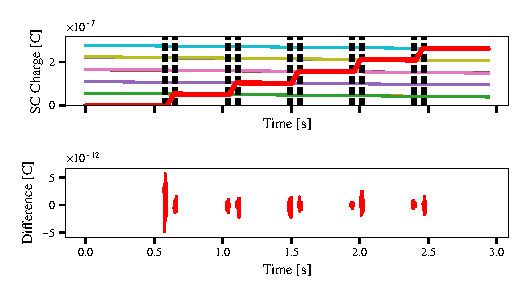
\includegraphics[width=\columnwidth]{sc_reduc_966}
\caption{Solar cell charge sequence reduction process at wavelength $\lambda_L=\SI{469}{\nm}$. Pairs of vertical black at the left and right of a burst encompass the fitted dark sequences. Coloured curves are the dark model fitted within these dark times. The top panel shows the raw charges acquired with the solar cell, while the bottom panel shows the residuals to the dark model fit during dark times only.}\label{fig:sc_reduc}
\end{figure}

As for the photodiode, we modelled the dark sequence before and after each burst. The solar cell dark model is the sum of a linear function plus two sinus functions at fixed frequency \SI{50}{\hertz} and \SI{100}{\hertz}:
\begin{align}
    q_{\rm solar}^{\rm dark}(t) = a_{\rm solar}t + b_{\rm solar} & + A_{50} \sin \left( 100 \pi t + \phi_{50}\right)  \notag \\  & +  A_{100} \sin \left( 200 \pi t + \phi_{100}\right)
\end{align}
where $a_{\rm solar}, b_{\rm solar}, A_{50}, A_{100}, \phi_{50}$ and $\phi_{100}$ are free parameters fitted on data. 
Again, we call $t_1$ and $t_2$ the time stamps of the beginning and end of the laser burst, respectively, given by the laser trigger output itself.
The accumulated charge $\Qsolarmes$ during a burst is then
\begin{align}\label{eq:qsolar}
\Qsolarmes  = & q_{\rm solar,2}^{\rm dark}(t_2) - q_{\rm solar, 1}^{\rm dark}(t_1) \\  &  - \frac{1}{2} \left[q_{\rm solar,1}^{\rm dark}(t_2) - q_{\rm solar,1}^{\rm dark}(t_1) + q_{\rm solar,2}^{\rm dark}(t_2) - q_{\rm solar,2}^{\rm dark}(t_1)  \right]    \notag
\end{align}
where the indices $1$ and $2$ refer again to data before and after the burst, respectively. The purpose of the term in brackets is to subtract an estimation of the dark current contribution during the burst itself. Free $q_{\rm solar}^{\rm dark}(t)$ parameters were fitted, minimising a $\chi^2$ with a Newton-Raphson gradient descent. Power lines are well fitted by the model (no more periodic oscillations in the residuals) as shown in Figure~\ref{fig:sc_reduc_zoom} where $A_{50}$ was about $\SI{50}{\pico\coulomb}$.
The $1/f$ noise is not modelled in $q_{\rm solar}^{\rm dark}(t)$ as it is subdominant, but the lowest frequency modes are captured by the values of $a_{\rm solar}$ and $b_{\rm solar}$. To get a close estimate of their contributions during the burst, we fit the dark sequences only during $\tau_b/2$ around the burst to rely on their extrapolation inside the burst window (with a minimum of 12 data points to encompass at least one \SI{50}{\hertz} period). %Doing so, both linear functions are the sum of both darks containing the same $1/f$ noise power as during the laser burst and only the long-wave modes that pollute the laser burst.
Indeed, as exhibited in Figure~\ref{fig:sc_reduc_zoom}, fits of $q_{\rm solar,2}^{\rm dark}(t)$ after the first burst (orange) and of $q_{\rm solar,1}^{\rm dark}(t)$ before the second burst (green) do not superimpose because of the long-range $1/f$ noise that deviates the data from a global linear relationship. So focusing the fits in two windows of size $\max(\SI{22}{\ms},\tau_b/2)$ permits to capture contaminating $1/f$ modes no longer than $\tau_b$. 

Charge value $\Qsolarmes$ is then computed for each laser burst following Equation~\ref{eq:qsolar}. Concerning estimating its statistical uncertainties $\Ssolarstat$, we add in quadrature the contributions from the parameter covariance matrix and the RMS of the residuals (to account for uncaptured $1/f$ modes). We trained the fitting procedure on pure dark data and noticed that $\Ssolarstat$ was too small to account for $\Qsolar^{\rm dark}$ null measurement dispersion. The RMS of the pull distributions was linearly dependent on the burst duration $\tau_b$, showing $\Ssolarstat$ did not capture all the long-range $1/f$ noise. Therefore, we corrected all $\Ssolarstat$ values with a multiplicative factor dependent on $\tau_b$. Doing so, we found an unbiased null measurement $\Qsolar^{\rm dark}$ with a pull distribution of RMS $\;\approx 1$ whatever the burst duration $\tau_b$ (Figure~\ref{fig:charge_pull}). 

%cbp_paper_plots.py
\begin{figure}[!h]
\centering
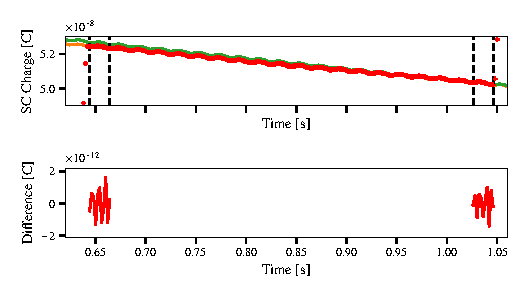
\includegraphics[width=\columnwidth]{sc_reduc_966_zoom}
\caption{Same as Figure~\ref{fig:sc_reduc} but zoomed on the second dark sequence. The orange model is fitted on dark data on the left of the plot, while the green model is fitted on dark data on the right.}\label{fig:sc_reduc_zoom}
\end{figure}


\subsubsection{Spectrograph data reduction overview}
\label{sec:spectro_reduction}

The spectrograph exposure times were adjusted to avoid the saturation level for all wavelengths. However, the sampling rate was not tunable, and time stamps were unavailable. So we took as many spectra $N(\lambda_p)$ as possible during an acquisition and then analysed them. Some contained laser light, and others were darks. We assumed a spectrum is dark if there are no spectrograph pixels above its median plus a threshold in the region around the laser wavelength. This algorithm works for most spectra except for very weak laser lines that come too close to a hot pixel, but very rarely.

After this sorting of the spectra in two categories ("laser on" and "laser off"), we subtract the master bias $B(\lambda_p)$ and compute a master dark spectrum $D(\lambda_p)$, taking the median of all the dark spectra. This master dark is subtracted from all spectra. This removes the spectrograph baseline and hot pixels. The spectra containing laser lines are stacked to increase the signal-to-noise ratio. Let's call $S(\lambda_p)$ the stacked spectrum after bias and dark subtraction:
\begin{align}
D(\lambda_p) & = \sum_{i \in \left\lbrace \text{laser off}\right\rbrace}\left( N_i(\lambda_p) - B(\lambda_p)\right), \\
    S(\lambda_p) & = \sum_{i \in \left\lbrace \text{laser on}\right\rbrace}\left( N_i(\lambda_p) - D(\lambda_p) - B(\lambda_p)\right).
\end{align}
The spectrograph error model is applied to get the intensity uncertainties $\sigma_p$ for each spectrum $i$:
\begin{equation}\label{eq:spectro_error_model_data}
\sigma^2_{i,p} =\sigma_{ro}^2 +  (N_i(\lambda_p) - B(\lambda_p))/G + \sigma_G^2 (N_i(\lambda_p) - B(\lambda_p))^2
\end{equation}
As the signal-to-noise in the stacked spectrum is very high, we assimilate the $S(\lambda_p)$ value to its empirical average to get $\sigma_{i,p}$. The uncertainties are propagated to the stacked spectrum $S(\lambda_p)$.

Then, to detect emission lines in $S(\lambda_p)$, we fit locally Gaussian profiles on top of a linear background. The $\lambda_g$ fit is unweighted as for the spectrograph calibration process. We searched for the laser line and lines at \SI{532}{\nm} and from two-photon conversions. Indeed, we noticed the presence of a \SI{532}{\nm} line in the regime 532 to \SI{669}{\nm} and of a weak line when the laser is set to wavelength above \SI{1064}{\nm}. If we call $\lambda_L$ the wavelength at which the laser was set, we observed the production of photons at wavelength $\lambda_{\text{comp}}$, which seems given by
\begin{equation}
 \frac{2}{\SI{1064}{\nm}} \approx \frac{1}{\lambda_L} + \frac{1}{\lambda_{\text{comp}}}
 \end{equation} 
due to the conversion of two \SI{1064}{\nm} photons into a laser photon at $\lambda_L$ and a complementary photon at $\lambda_{\text{comp}}$ that ended in the laser beam. In practice, we observed a small emission line in the spectrograph when $\lambda_L > \SI{1064}{\nm}$, nearly symmetrical of the laser line with respect to \SI{1064}{\nm}. 

An example of a stacked spectra with the detection of the laser line at \SI{643}{\nm} and the pump line at \SI{532}{\nm} is shown in Figure~\ref{fig:spectro_reduc_643}, before spectrograph wavelength calibration. The average intensity value far from the emission lines is zero, with statistical error bars compatible with the observed dispersion. Intensity uncertainties are propagated up to the line centroid wavelength. 

%cbp_paper_plots.py
\begin{figure}[!h]
\centering
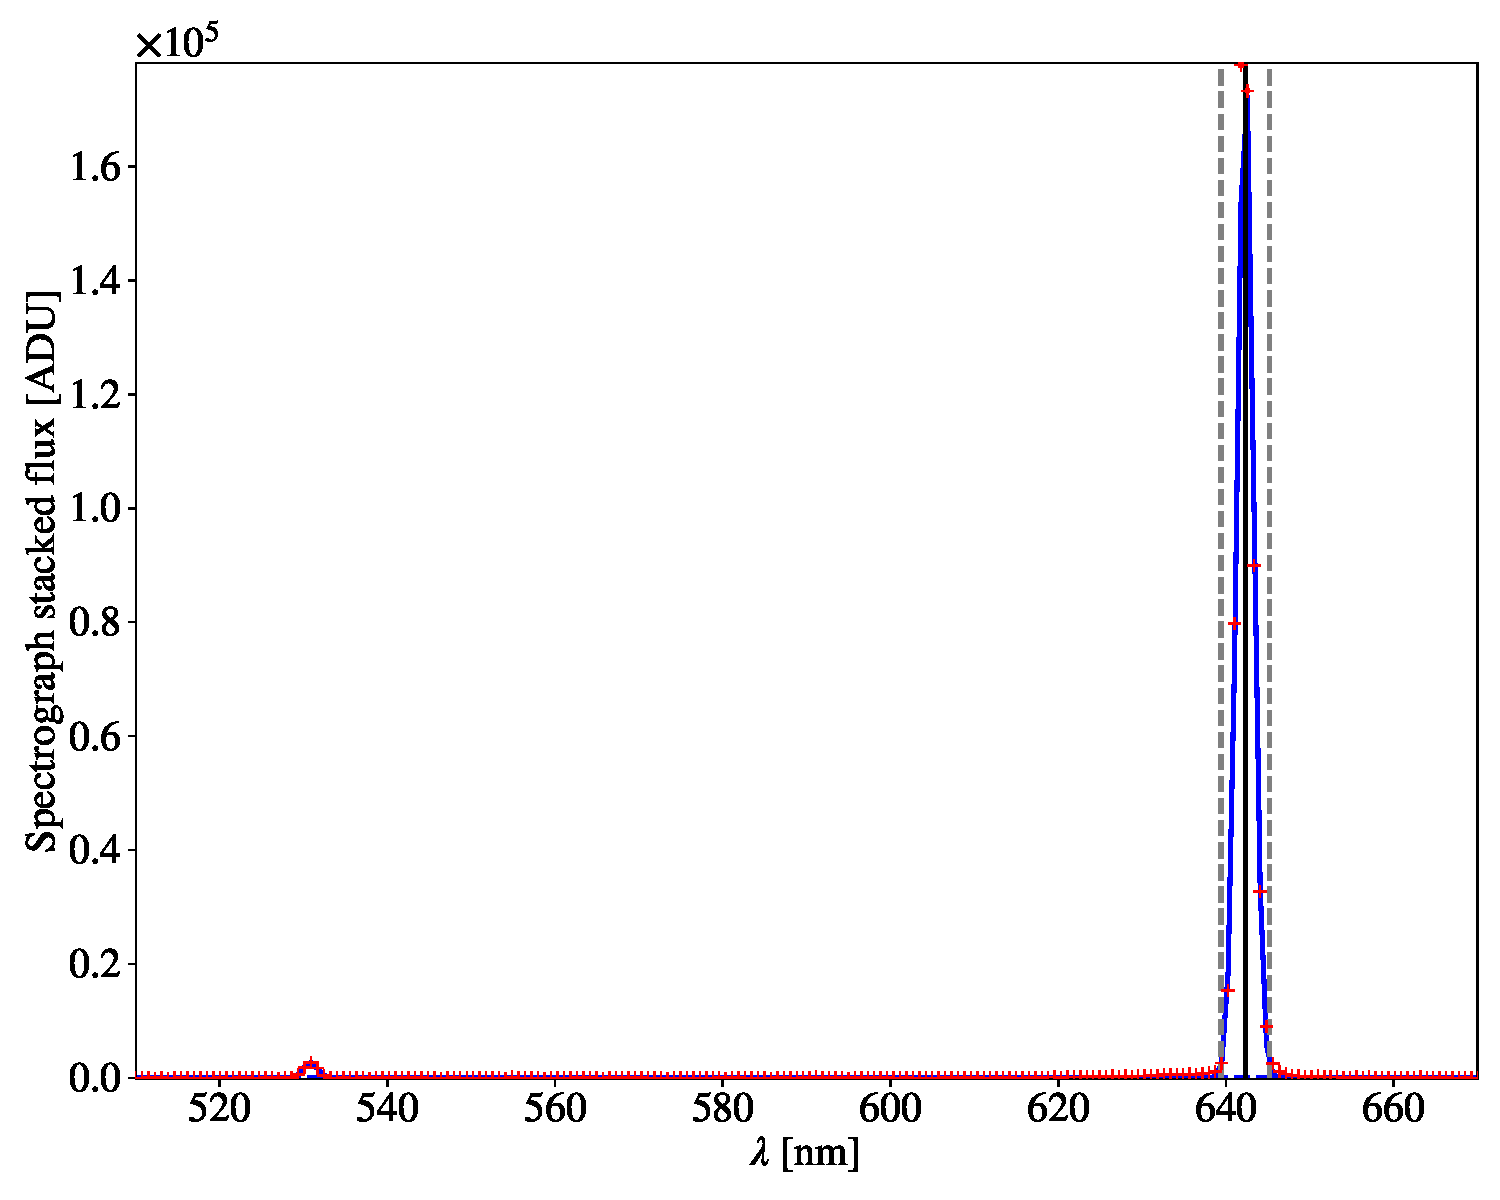
\includegraphics[width=\columnwidth]{spectro_reduc_643}
\caption{Fit of Gaussian profiles (blue lines) in the stacked spectra (red dots) for a laser line set at $\lambda_L=\SI{643}{\nm}$, with raw spectrograph wavelengths on the abscissa axis. The contamination line at \SI{532}{nm} is also visible. The black vertical line gives the fitted laser line centroid. The grey vertical lines delimit a region of $\pm 3\sigma_g$ around the centroid, where $\sigma_g$ is the fitted RMS of the Gaussian profile. The total laser flux is the sum of the pixel values in this region.}\label{fig:spectro_reduc_643}
\end{figure}

We used the \SI{532}{\nm} line to check the quoted statistical errors $\sigma_\lambda^{\rm noise}$ on wavelength. For all data sets, we plotted the fitted line position versus time. The RMS is compatible with the quoted error bars on wavelength for lower signal-to-noise ratio data sets. But for the high signal-to-noise ratio data sets, some dispersion is unaccounted, explained by the fact that the Gaussian profile is an incomplete model of high signal-to-noise lines. Therefore, we added a $\sigma_\lambda^{\rm PSF}=\SI{0.012}{\nm}$ statistical uncertainty due to PSF modelling on wavelength uncertainty to get a normal distribution for the residuals normalised by the full statistical uncertainties (see Figure~\ref{fig:wavelength_error_model_consistency}), the latter being
\begin{equation}
    \left(\sigma_{\lambda}^{\rm stat}\right)^2 =  \left(\sigma_{\lambda}^{\rm noise}\right)^2 +  \left(\sigma_{\lambda}^{\rm PSF}\right)^2.
\end{equation}

%cbp_paper_plots.py
\begin{figure}[!h]
\centering
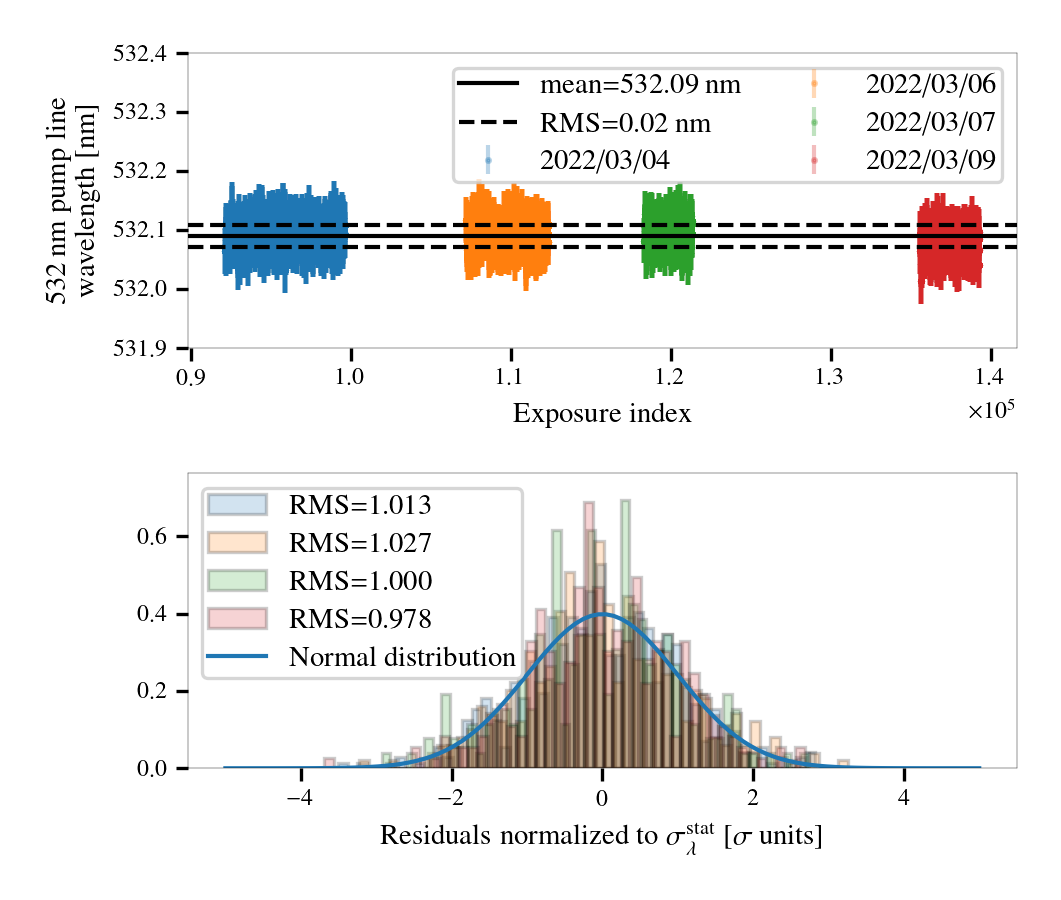
\includegraphics[width=\columnwidth]{wavelength_error_model_consistency.png}
\caption{Top: all measured \SI{532}{\nm} pump line calibrated wavelengths with respect to exposure index ($\approx\num{250000}$ data points) for the four solar cell runs. Bottom: distributions of residuals to the mean wavelength normalized by $\sigma_{\lambda}^{\rm stat}$ (colored bars) with RMS quoted in legend. A normal distribution of RMS 1 is overplotted for comparison.}\label{fig:wavelength_error_model_consistency}
\end{figure}

Finally, the spectrograph wavelength calibration is applied to detected wavelengths, and corresponding systematic uncertainty is added. The final quoted wavelength is $\lambda_c$ and the final wavelength uncertainty is
\begin{equation}
  \left(\sigma_{\lambda}\right)^2 =  \left(\sigma_{\lambda}^{\rm stat}\right)^2 +  \left(\sigma_{\lambda}^{\rm cal}\right)^2.   
\end{equation}
The composition of the final wavelength error budget is detailed in Section~\ref{sec:wavelength_syst}.

The laser line flux $\Qspectromain$, the \SI{532}{\nm} line flux $\Qspectro^{532}$ and the $\lambda_{\rm comp}$ line flux $\Qspectro^{\rm comp}$ flux are computed summing the pixels in a window of $\pm 3 \sigma_g$ where $\sigma_g$ is the RMS of the fitted Gaussian profile, after dark and bias subtraction. Associated statistical uncertainties are computed from the standard error propagation of the $\sigma_{i,p}$ values. These fluxes are used to correct solar cell and photodiode charges as well as the \SD photometry from the $\SI{532}{\nm}$ line contamination (see Section~\ref{sec:532_cont}).  %As the \SI{532}{\nm} line flux is always at most 1\% of the laser line flux,

\subsection{CBP ratio of charges}

A first CBP response estimation can be computed as $r_{\rm CBP}^{\rm mes} = \Qsolarmes/\Qphotmes$ to check the statistical uncertainties and then analyse systematic uncertainties. The ratio of charges is presented in Figure~\ref{fig:cbp_charge_ratio}. Each black point is a ratio of charge measurements from one burst at one wavelength $\lambda_L$. They follow a smooth curve in $\lambda_L$. The $r_{\rm CBP}^{\rm mes}$ statistical uncertainties 
\begin{equation}
    \sigma_{\mathrm CBP}^{\rm stat} = r_{\rm CBP}^{\rm mes} \sqrt{\left(\frac{\Ssolarstat}{\Qsolarmes}\right)^2 +  \left(\frac{\Sphotstat}{\Qphotmes}\right)^2 }
\end{equation}
are higher in the blue part as the laser is weaker in this regime (around $0.1\%$) than in the red part (around $0.01\%$). They were correctly estimated as the difference between all data points and a spline curve passing through the points, normalised by the statistical uncertainties, follows a Gaussian distribution of mean 0 and RMS$\;\approx 1$, as expected. If we compute a mean CBP response

%cbp_paper_plots.py
\begin{figure}[!h]
\centering
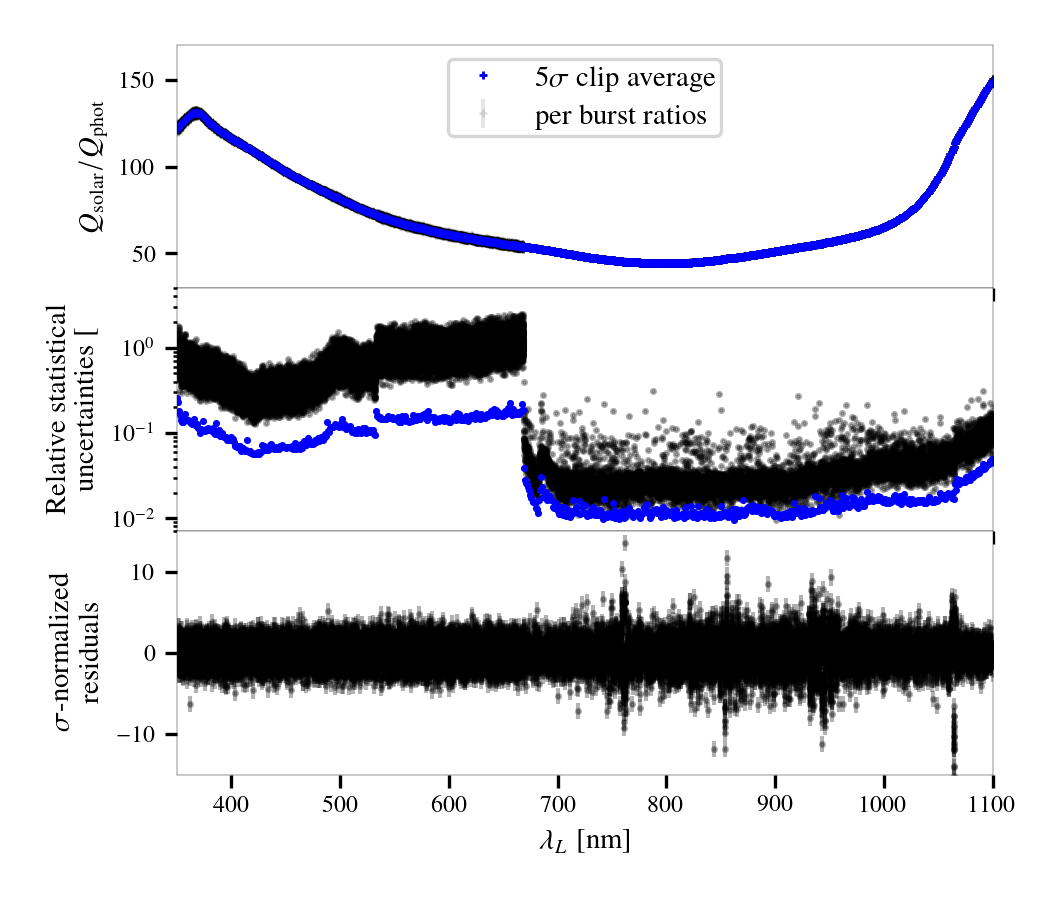
\includegraphics[width=\columnwidth]{fig/cbp_charge_ratio.png}
\caption{CBP charge ratio $\Qsolarmes/\Qphotmes$ as a function of $\lambda_L$. Top: every black point is a charge measurement ratio from one burst, the blue curve is the $5\sigma$-clipped average. Middle: relative uncertainties on $\Qsolarmes/\Qphotmes$. Bottom: pull distribution after spline subtraction.}\label{fig:cbp_charge_ratio}
\end{figure}


\subsection{Systematics}



\subsubsection{Wavelength calibration}\label{sec:wavelength_syst}

%cbp_paper_plots.py
\begin{figure}[!h]
\centering
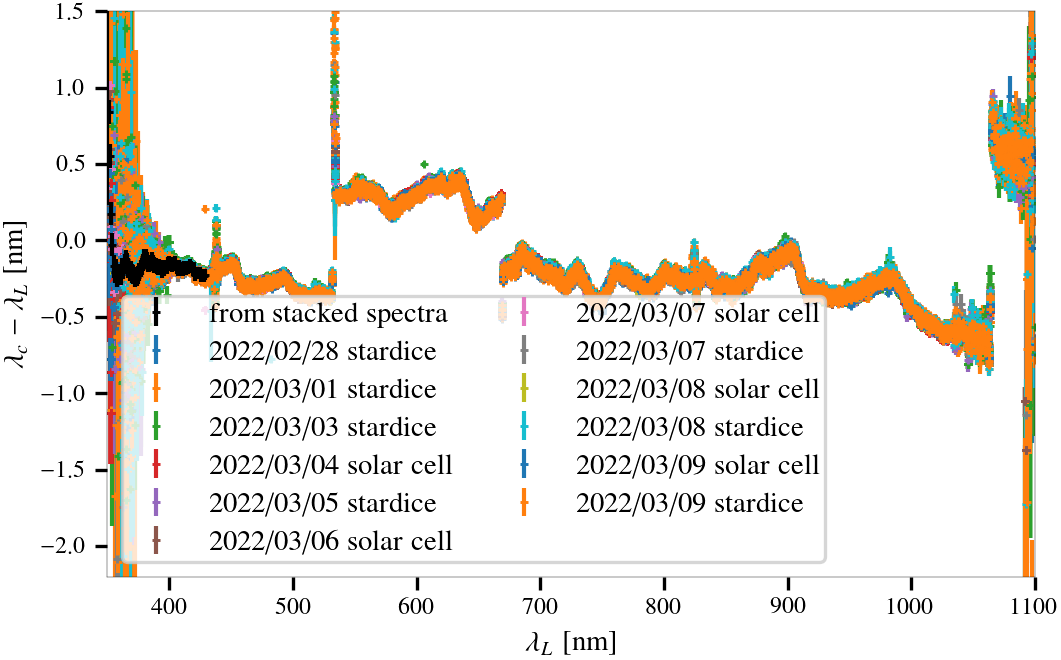
\includegraphics[width=\columnwidth]{wavelength_stability.png}
\caption{Difference between the calibrated $\lambda_c$ and requested laser wavelengths $\lambda_L$, for all the $\approx \num{350000}$ laser line wavelengths acquired during our measurement campaign.}\label{fig:wavelength_stability}
\end{figure}


The realised wavelength is never the one a priori asked, as shown in Figures~\ref{fig:sc_dataset_examples} and~\ref{fig:wavelength_stability}. However, we observed remarkable repeatability of the correspondence between the set wavelength $\lambda_L$ and the realised wavelength $\lambda_g$ in Figure~\ref{fig:wavelength_stability}. This figure represents every $\approx\num{350000}$ laser bursts shot and analysed during the CBP measurement campaign. The superimposition of all measurements at each laser wavelength $\lambda_L$ exhibits good stability of the laser with time and of the $\lambda_g$ wavelength fit with line intensity. The RMS is better than \SI{0.02}{\nm} at most wavelengths, except where line determination is ambiguous: close to the contamination lines at $\SI{532}{nm}$ and $\SI{1064}{nm}$, and close to the sensor edges. As the bijection between $\lambda_L$ laser wavelengths and realised wavelengths $\lambda_c$ is unambiguous, in some figures of this paper, we use the set laser wavelength $\lambda_L$ for clarity. 

Figure~\ref{fig:wavelength_error_budget} details the total error budget from wavelength calibration for three different runs: two runs shooting at StarDice with two pinholes and one run shooting at the solar cell. Uncertainty on wavelength $\sigma_\lambda$ is primarily dominated by wavelength calibration uncertainties in the range 400 to \SI{1080}{\nm}. Statistical uncertainty dominates around $\SI{532}{\nm}$ and close to the spectrograph sensor edges. Except in these cases, $\sigma_\lambda$ is well below $\SI{1}{\angstrom}$, which allows for precisely measuring the telescope filter band-passes better than the Angstrom level.   

\todo{Expliquer comment on propage les incertitudes de $\sigma_\lambda$ sur les résultats finaux.}

%cbp_paper_plots.py
\begin{figure}[!h]
\centering
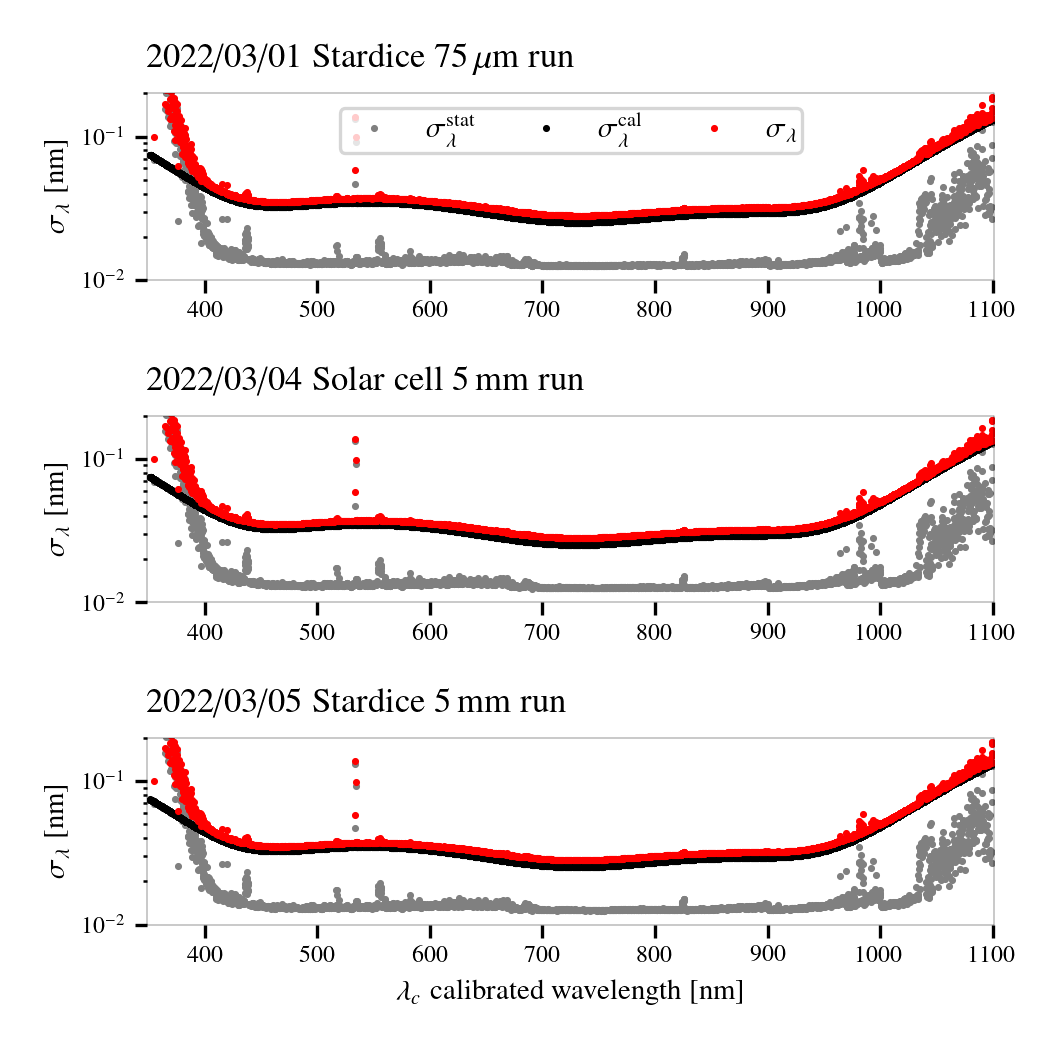
\includegraphics[width=\columnwidth]{spectrograph_error_budget.png}
\caption{Total error budget (red) of calibrated wavelengths $\lambda_c$ for three different runs (from top to bottom: StarDice run with \SI{75}{\um} pinhole, solar cell run with \SI{5}{mm} pinhole, StarDice run with \SI{5}{mm} pinhole) as a function of the laser set wavelength $\lambda_L$. Detection uncertainties (grey) represent PSF modelling uncertainties and Gaussian fit uncertainties, while calibration uncertainties (black) come from the Hg-Ar lamp calibration procedure. }\label{fig:wavelength_error_budget}
\end{figure}

To evaluate systematic uncertainty on the CBP response due to the wavelength calibration, we computed $r_{\rm CBP}$ at $\lambda_c+\sigma_{\lambda^{\rm cal}}$ and $\lambda_c-\sigma_{\lambda^{\rm cal}}$. The difference between both CBP responses is well below the statistical uncertainty, as the CBP response varies slowly in $\lambda$ whole $\sigma_\lambda$ is sub-Angstrom (see Figure~\ref{fig:cbp_charge_ratio}). The importance of $\sigma_\lambda$ as a systematic uncertainty lies essentially in the determination of the telescope filter band-passes and the position of their sharp edges.


\subsubsection{Ambient light}\label{sec:sc_linearity}

 %cbp_paper_plots.ipynb
\begin{figure}[h]
    \centering
    \includegraphics[width=\columnwidth]{fig/sc_dark_qswMAX.png}
    \caption{CBP charge ratio $\Qsolar^{\rm dark}/\Qphot^{\rm dark}$ as a function of $\lambda_L$: every black point is a charge measurement ratio from one burst, the blue curve is the $5\sigma$-clipped average.}
    \label{fig:sc_dark}
\end{figure}

To check contamination by ambient light, we ran a solar cell acquisition with a cap on the CBP telescope. In that way, the solar cell can collect indirect light from the laser box when firing. The measurement of this indirect ambient light $\Qsolar^{\rm dark}$ constitutes a "dark" for our CBP calibration. From this specific run, we built a dark CBP response $r_{\mathrm{CBP}}^{\rm dark} = \Qsolar^{\rm dark} / \Qphot^{\rm dark}$ where $\Qsolar^{\rm dark}$ (resp. $\Qphot^{\rm dark}$) is the burst charge collected in the solar cell (resp. the photodiode). For each $\lambda_L$, burst ratios are averaged with a $5\sigma$ clipping, giving the blue curve $r_{\mathrm{CBP}}^{\rm dark}(\lambda_L)$ in Figure~\ref{fig:sc_dark}. The dark contribution in our solar cell data is then evaluated as follows:
\begin{equation}
    \Qsolar^{\rm dark} = r_{\mathrm{CBP}}^{\rm dark}(\lambda_L) \times \Qphotmes(\lambda_L)
\end{equation}
and subtracted from all our measurements. This correction is the main contribution to instrumental non-linearity we identified. 


\subsubsection{Laser light contamination}
\label{sec:532_cont}

As described in Section~\ref{sec:cbp}, the light source used is a tunable laser using a pump laser at \SI{532}{\nano\meter}, which has different regimes. When we operated within the range [532 - 644] nm, in the spectrograph, we observed a contamination light at \SI{532}{\nano\meter} for all wavelengths in this range. 

We must account for this light contamination to get the true amount of charges $\Qsolarcal$ coming from main laser line. Therefore, we built a model for the \SI{532}{\nano\meter} contribution observed in the range [532 - 644] nm. The total charge measured in the solar cell $\Qsolarmes$ is the sum of the charges from the main wavelength $\lambda_L$ and the charges from contaminations, like the \SI{532}{\nm} contamination. This is the same for the total charges measured in the photodiode $\Qphotmes$ with $\Qphot$ and $\Qphot^{532}$ respectively the charges from the main laser line and the charges from the \SI{532}{\nm} contamination:
\begin{align}
%\Qsolarmes(\lambda_L) & = \Qsolar(\lambda_L) + \Qsolar^{532}(\lambda_L) + r_{\mathrm{CBP}}^{\rm dark}(\lambda_L) \times \Qphotmes(\lambda_L) \label{eq:qsolar_mes} \\
\Qphotmes(\lambda_L) & = \Qphot(\lambda_L) + \Qphot^{532}(\lambda_L) \label{eq:qphot_mes}
\end{align}

In the spectrograph, we measured two fluxes from two separated peaks: the one from the main wavelength $\Qspectromain$, and the one from the \SI{532}{\nm} contamination $\Qspectro^{532}$. As the light is homogeneous in the integrating sphere, the proportion of contamination light and laser light is the same at the entrance of both instruments. This translates into the equality
\begin{equation}
    \frac{\Qspectro^{532}}{\Qspectromain} \times \frac{\Espectro(\lambda_L)}{\Espectro(532)} = \frac{\Qphot^{532}}{\Qphot} \times \frac{\Ephot(\lambda_L)}{\Ephot(532)}
    \label{eq:prev_alpha}
\end{equation}
where $\Ephot(\lambda_L)$ and $\Espectro(\lambda_L)$ are the quantum efficiencies of the photodiode and the spectrograph sensor with its optical fiber, respectively. Their values can be taken from manufacturer data sheets (Figure~\ref{fig:QEs}), or their ratio
\begin{equation}\label{eq:eta}
\eta(\lambda) = \frac{\Espectro(\lambda)}{\Ephot(\lambda)} = \frac{\Qspectromain(\lambda)}{\Qphot(\lambda)}
\end{equation}
can be measured directly with all our measurements in spectrograph ADU per photodiode unit (Figure~\ref{fig:QEs}). In the following, we used the estimate of $\eta(\lambda)$ instead of the vendor curves, with an uncertainty given by its RMS around a smooth spline curve.

Then, we defined the $\alpha(\lambda)$ ratio function as
\begin{equation}
    \alpha(\lambda_L) = \frac{\Qphot^{532}(\lambda_L)}{\Qphot(\lambda_L)} = \frac{\Qspectro^{532}(\lambda_L)}{\Qspectromain(\lambda_L)} \times \frac{\Espectro(\lambda_L)\Ephot(532)}{\Ephot(\lambda_L)\Espectro(532)} 
    \label{eq:alpha}
\end{equation}
to compute the level of contamination in the photodiode $\Qphot^{\lambda_L}/\Qphot^{532}$.

%cbp_paper_plots.py
\begin{figure}[h]
    \centering
    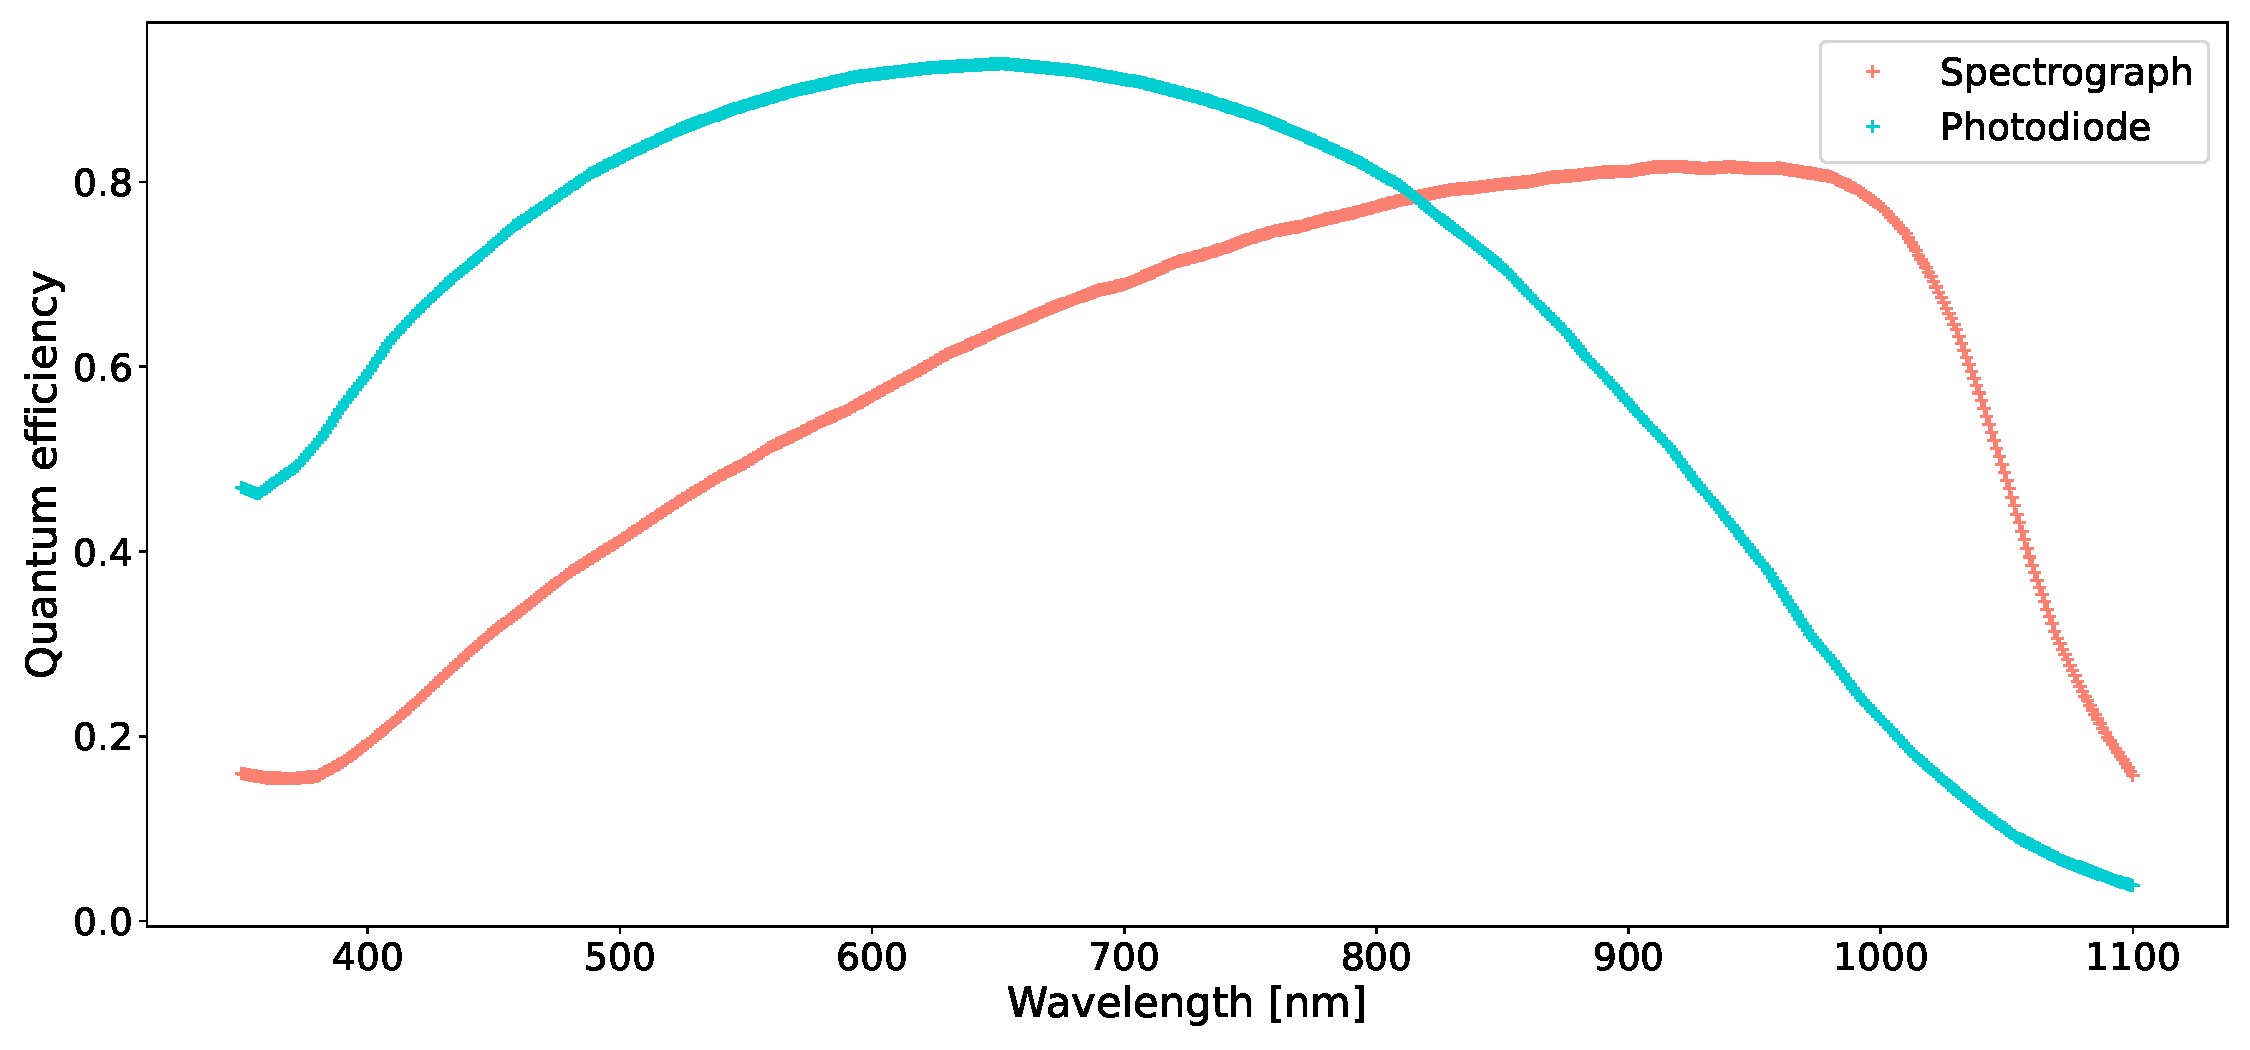
\includegraphics[width=\columnwidth]{fig/qe_phototiode_spectro.pdf}
    \caption{Quantum efficiencies of the spectrograph (red) and the photodiode (cyan), with the $\eta(\lambda)$ ratio (black).}
    \label{fig:QEs}
\end{figure}
    
We measured the $\alpha(\lambda_L)$ ratio with the right-hand side of Equation~\ref{eq:alpha} at every wavelength with the spectrograph data (Figure~\ref{fig:alpha_532}). We accumulated all available data with $\sigma_c < \SI{0.1}{\nm}$ (to reject data sets with confusion with the \SI{532}{\nm} line and the main laser line). We fitted a first degree polynomial function on all the $\Qspectro^{532}(\lambda_L)$ data points we had to allow us for a reasonable extrapolation in the range 532 - \SI{540}{\nm} where unambiguous data are missing. Uncertainties on  $\Qspectro^{532}$. Then, we computed the ratio $\alpha(\lambda_L)$ with that model for $\Qspectro^{532}$. It gives a rather flat curve between 540 and \SI{644}{\nm} of about 1\%, with smaller wiggles. Uncertainties are propagated in the extrapolation range using the standard error propagation formula, taking into account the covariances between the 2 model parameters. With this $\alpha$ model, we deduced the true photodiode charges coming from the main laser line at $\lambda_L$
\begin{equation}
        \Qphotcal(\lambda_L) \equiv  \frac{\Qphotmes(\lambda_L)}{1 + \alpha(\lambda_L)} \quad\text{if}\ \lambda_L \in \left[532, 644\right]\mathrm{\,nm}\label{eq:qphot_cal532}
\end{equation}
We introduce here the notation $\Qphotcal$ as the final calibrated amount of charges detected in the photodiode per laser burst. 

Light detected by the solar cell has gone through the CBP optics, with a response $\Rcbp$.
Then, the contribution of the \SI{532}{\nano\meter} photons collected by the solar cell is computed as
\begin{equation}
\begin{aligned}
    \Qsolar^{532}(\lambda_L) & = \Rcbp(532)  \Qphot^{532}(\lambda_L) \\ 
    & = \Rcbp(532) \frac{ \alpha(\lambda_L) }{1+ \alpha(\lambda_L)} \Qphotmes(\lambda_L).
    \label{eq:qsolar_cal532}
\end{aligned}
\end{equation}
Thanks to the spectrograph data, using Equations~\ref{eq:qphot_cal532} and~\ref{eq:qsolar_cal532}, we can correct all our measurements from the \SI{532}{\nano\meter} in both the photodiode and the solar cell. The impact of this correction is illustrated in Section~\ref{sec:cbp_summary}.


\begin{figure}[h]
    \centering
    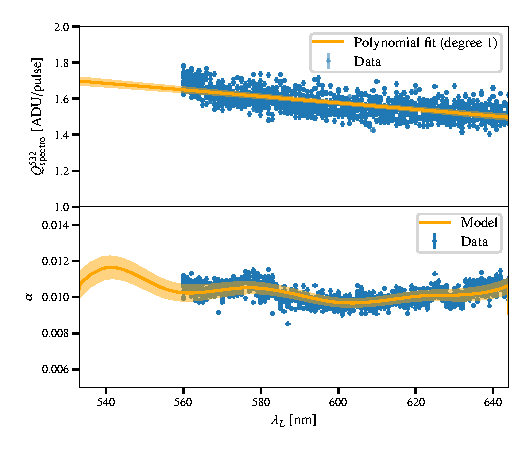
\includegraphics[width=\columnwidth]{fig/alpha_532_qswMAX.pdf}
    \caption{Top: all available data points for $\alpha$ computed from the spectrograph measurements (blue crosses) and degree 9 polynomial fit (orange) with its uncertainty (shaded orange band). Bottom: difference between data and model.}
    \label{fig:alpha_532}
    %~/stardice/analysis/cbp_paper/golden_sample_analysis/dr3/532nm_correction.ipynb
\end{figure}


We did the same correction for the complementary wavelength line $\lambda_{\rm comp}$ appearing after $\lambda_L > \SI{1064}{\nm}$. The correction coefficient $\beta$ analogue to $\alpha$ is
\begin{equation}
    \beta(\lambda_L) = \frac{\Qphot^{\lambda_{\rm comp}}(\lambda_L)}{\Qphot(\lambda_L)} = \frac{\Qspectro^{\lambda_{\rm comp}}(\lambda_L)}{\Qspectromain(\lambda_L)} \times \frac{\Espectro(\lambda_L)\Ephot\contcomp}{\Ephot(\lambda_L)\Espectro\contcomp} 
    \label{eq:beta}
\end{equation}
and is represented Figure~\ref{fig:beta}. The $\Qspectro^{\lambda_{\rm comp}}$ data points were modelled by a degree 1 polynomial function to allow us extrapolating $\beta$ in the range [1064 - 1070]\,nm. Similarly, the calibrated amount of charges in the photodiode corrected from the $\lambda_{\rm comp}$ photons is
\begin{equation}
        \Qphotcal(\lambda_L) \equiv  \frac{\Qphotmes(\lambda_L)}{1 + \beta(\lambda_L)} \quad\text{if}\ \lambda_L > \SI{1064}{\nano\meter}
        \label{eq:qphot_cal1064}
\end{equation}
and their contribution $\Qsolar^{\lambda_{\rm comp}}$ in the solar cell is given by
\begin{equation}
\begin{aligned}
    \Qsolar^{\lambda_{\rm comp}}(\lambda_L) & = \Rcbp(\lambda_{\rm comp})  \Qphot^{\lambda_{\rm comp}}(\lambda_L) \\ 
    & = \Rcbp(\lambda_{\rm comp}) \frac{ \beta(\lambda_L) }{1+ \beta(\lambda_L)} \Qphotmes(\lambda_L).
    \label{eq:qsolar_cal1064}
\end{aligned}
\end{equation}

Both corrections' impact is illustrated in Section~\ref{sec:sc_linearity} and Figure~\ref{fig:SCqswlinearity}, and Section~\ref{sec:sd_contaminations}.


\begin{figure}[h]
    \centering
    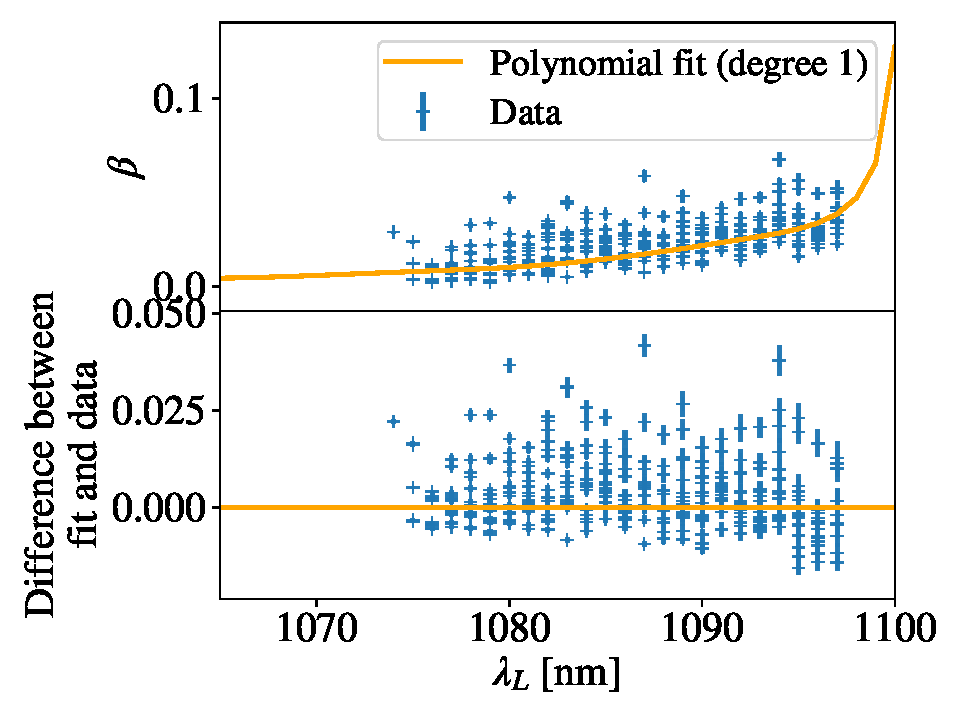
\includegraphics[width=\columnwidth]{fig/beta_532_qswMAX.pdf}
    \caption{Same as Figure~\ref{fig:alpha_532} but for $\beta$ correction coefficient.}
    \label{fig:beta}
    %~/stardice/analysis/cbp_paper/golden_sample_analysis/dr3/1064nm_correction.ipynb
\end{figure}


\subsubsection{Integrating sphere fluorescence}\label{sec:fluorescence}


\begin{figure}[h]
    \centering
    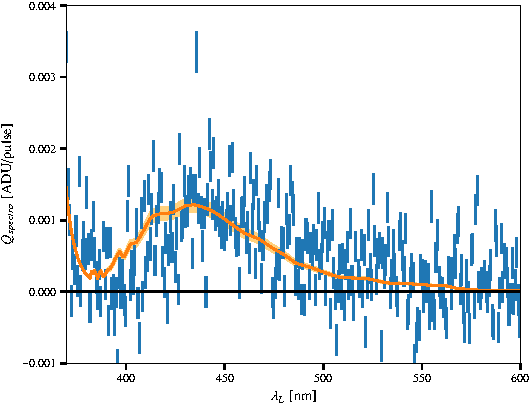
\includegraphics[width=\columnwidth]{fig/spectro_stack_fluo_model.pdf}
    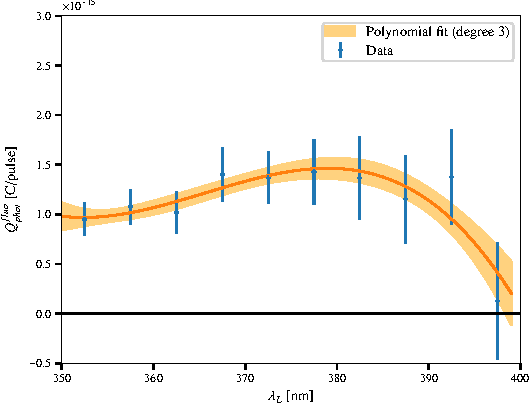
\includegraphics[width=\columnwidth]{fig/QPDfluo_model.pdf}
    \caption{Top: integrating sphere fluorescence spectrum from a stack of all solar cell run data with $\lambda_L < \SI{370}{\nano\meter}$ (blue crosses), with the best-fit model (orange line). Bottom: estimated fluorescence contribution in photodiode measured charges $\Qphot^{\rm fluo}$ as a function of wavelength (blue crosses) with a fitted third-order polynomial function (orange line).}
    \label{fig:fluo}
    %~/stardice/analysis/cbp_paper/golden_sample_analysis/dr3/1064nm_correction.ipynb
\end{figure}

Our integrating sphere appeared to be fluorescent at laser wavelengths below \SI{400}{\nano\meter}. The fluorescence of integrating spheres is studied in~\cite{shaw2007ultraviolet}. The fluorescent signal is visible in the \SD camera using the g filter or the grating but is very weak in the spectrograph. To visualise and model it, we stacked all our spectra per bins of \SI{5}{\nano\meter} in $\lambda_L$ (Figure~\ref{fig:fluo} top). The fluorescence signal spans a range of wavelength between $\approx \SI{400}{\nano\meter}$ and $\approx\SI{500}{\nano\meter}$, with an emission peak around with a emission peak at \SI{450}{\nano\meter}. %The peak amplitude depends on the laser wavelength, as expected for a fluorescence phenomenon. 

To estimate the contamination from fluorescence photons, we fitted a fluorescence spectrum model taken from Figure~9 of \cite{shaw2007ultraviolet}, with a constant background and a Moffat profile for the laser line for each stacked spectra. The fluorescence spectrograph flux is converted into photodiode charges $\Qphot^{\mathrm{fluo}}$ using the $\eta(\lambda)$ conversion factor and normalised by the total number of laser pulses (Figure~\ref{fig:fluo} bottom)\footnote{Contrary to the \SI{532}{\nano\meter} line contamination correction, we can not normalise by the flux in the main laser line as it is often noise-dominated in un-stacked spectra when $\lambda_L < \SI{400}{\nano\meter}$.}. We observed that the fluorescence spectrum cancels at $\lambda_L \geq \SI{400}{\nano\meter}$. So, for every wavelength $\lambda_L < \SI{400}{\nano\meter}$, we evaluate and subtract the contribution from the fluorescence contamination in the photodiode using the $\Qphot^{\mathrm{fluo}}(\lambda_L)$ model from Figure~\ref{fig:fluo}:
\begin{equation}
        \Qphotcal(\lambda_L) \equiv  \Qphotmes(\lambda_L) - \Qphot^{\mathrm{fluo}}(\lambda_L) \quad\text{if}\ \lambda_L < \SI{400}{\nano\meter}
        \label{eq:qphot_calfluo}
\end{equation}
We perform identically for $\Qsolarmes$ multiplying by the CBP response at \SI{450}{\nano\meter}: 
\begin{equation}
\begin{aligned}
    \Qsolar^{\rm fluo}(\lambda_L) & = \Rcbp(450)  \Qphot^{\rm fluo}(\lambda_L)
    \label{eq:qsolar_calfluo}
\end{aligned}
\end{equation}

This correction's impact is illustrated later in Section~\ref{sec:sd_contaminations}.

After the fluorescence, \SI{532}{\nano\meter} and $\lambda_{\mathrm{comp}}$ corrections, we updated our $\eta(\lambda)$ estimate and iterated several times to refine the light contamination subtractions.


\subsubsection{Instrumental chain linearity check}\label{sec:sc_linearity}
For the two solar cell runs we undertook, we varied the laser output power by a factor of around 2, namely, QSW at maximum and QSW set at 298. The ratio of the two CBP charge ratios before and after dark subtraction is presented in Figure~\ref{fig:SCqswlinearity}. Basically, no corrections lead to a ~5 permil deviations of the two CBP responses with respect to wavelength. Both CBP responses agree at $\approx 0.5\,$permil for wavelengths above \SI{669}{\nano\meter} when applying dark subtraction. Then, laser contamination correction makes the two CBP responses agree in the [532, 669]\,nm range better than 0.1 permil.

To assess the value of systematic uncertainties on the CBP response due to non-linearities, we take the absolute distance of the binned ratio to unity in four different ranges of wavelengths after dark subtraction and laser contamination correction (red segments in the bottom plot of Figure~\ref{fig:SCqswlinearity}).

%cbp_paper_plots.ipynb
\begin{figure}[h]
    \centering
    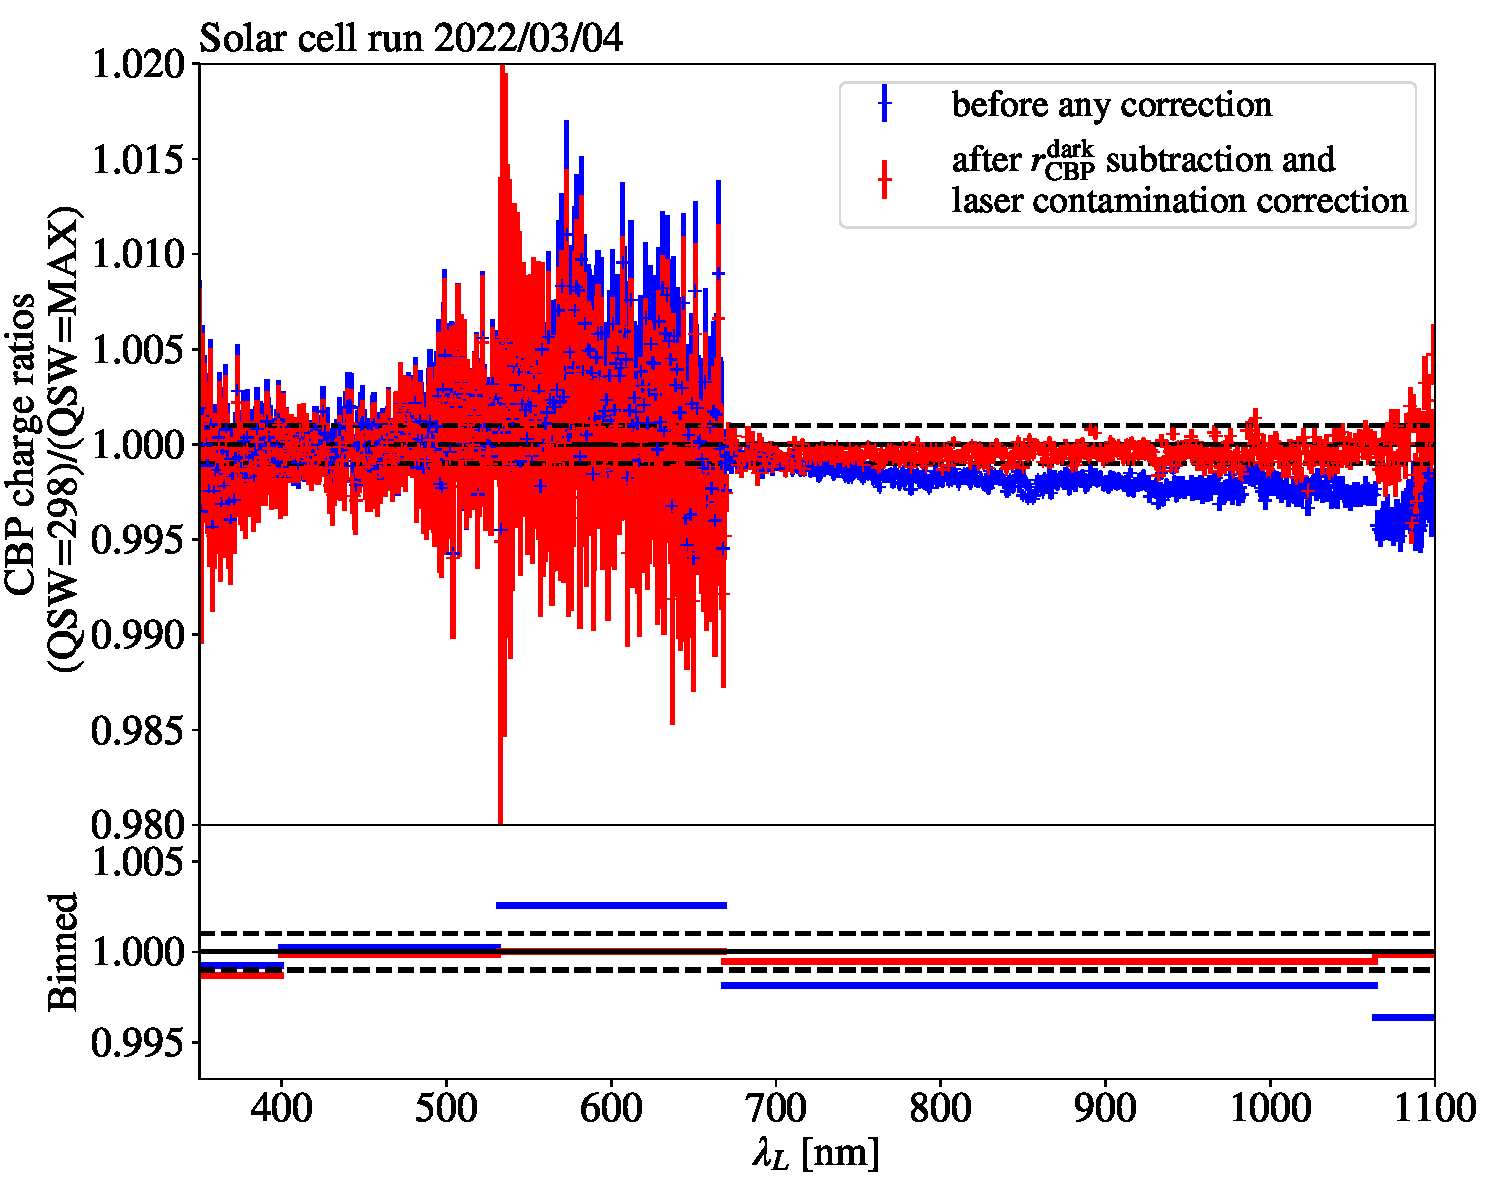
\includegraphics[width=\columnwidth]{fig/sc_qsw_ratios.pdf}
    \caption{Ratios of the CBP charge ratio for two different QSW values as a function of $\lambda_L$ coming from the 2022/03/04 solar cell run. Blue is for raw data while red is used for data corrected by dark contribution and laser contaminations. Black dashed lines encompass the permil precision region. Top: ratios for each $\lambda_L$. Bottom: binned ratio for four different wavelength ranges. A similar plot is obtained for the 2022/03/06 solar cell run.}
    \label{fig:SCqswlinearity}    
\end{figure}


\subsubsection{CBP scattered light varying the solar cell distance}

To measure the influence of scattered light in the CBP beam, we measured the CBP throughput by putting the solar cell \SI{16}{\cm} farther and compared it to the initial value. At this new position, we measured again the CBP dark from solar cell $\Qsolar^{\rm dark}$. Dark subtraction and laser contamination correction are applied. The comparison of both transmissions is presented in Figure~\ref{fig:sc_distance}. There is a decrease of the total light of about 3\textperthousand\ with a chromatic effect of about 2.5\textperthousand\ difference between \SI{350}{\nano\meter} and \SI{1100}{\nano\meter}. This constitutes the dominant systematics in the CBP throughput measurement.

%cbp_paper_plots.ipynb
\begin{figure}[h]
    \centering
    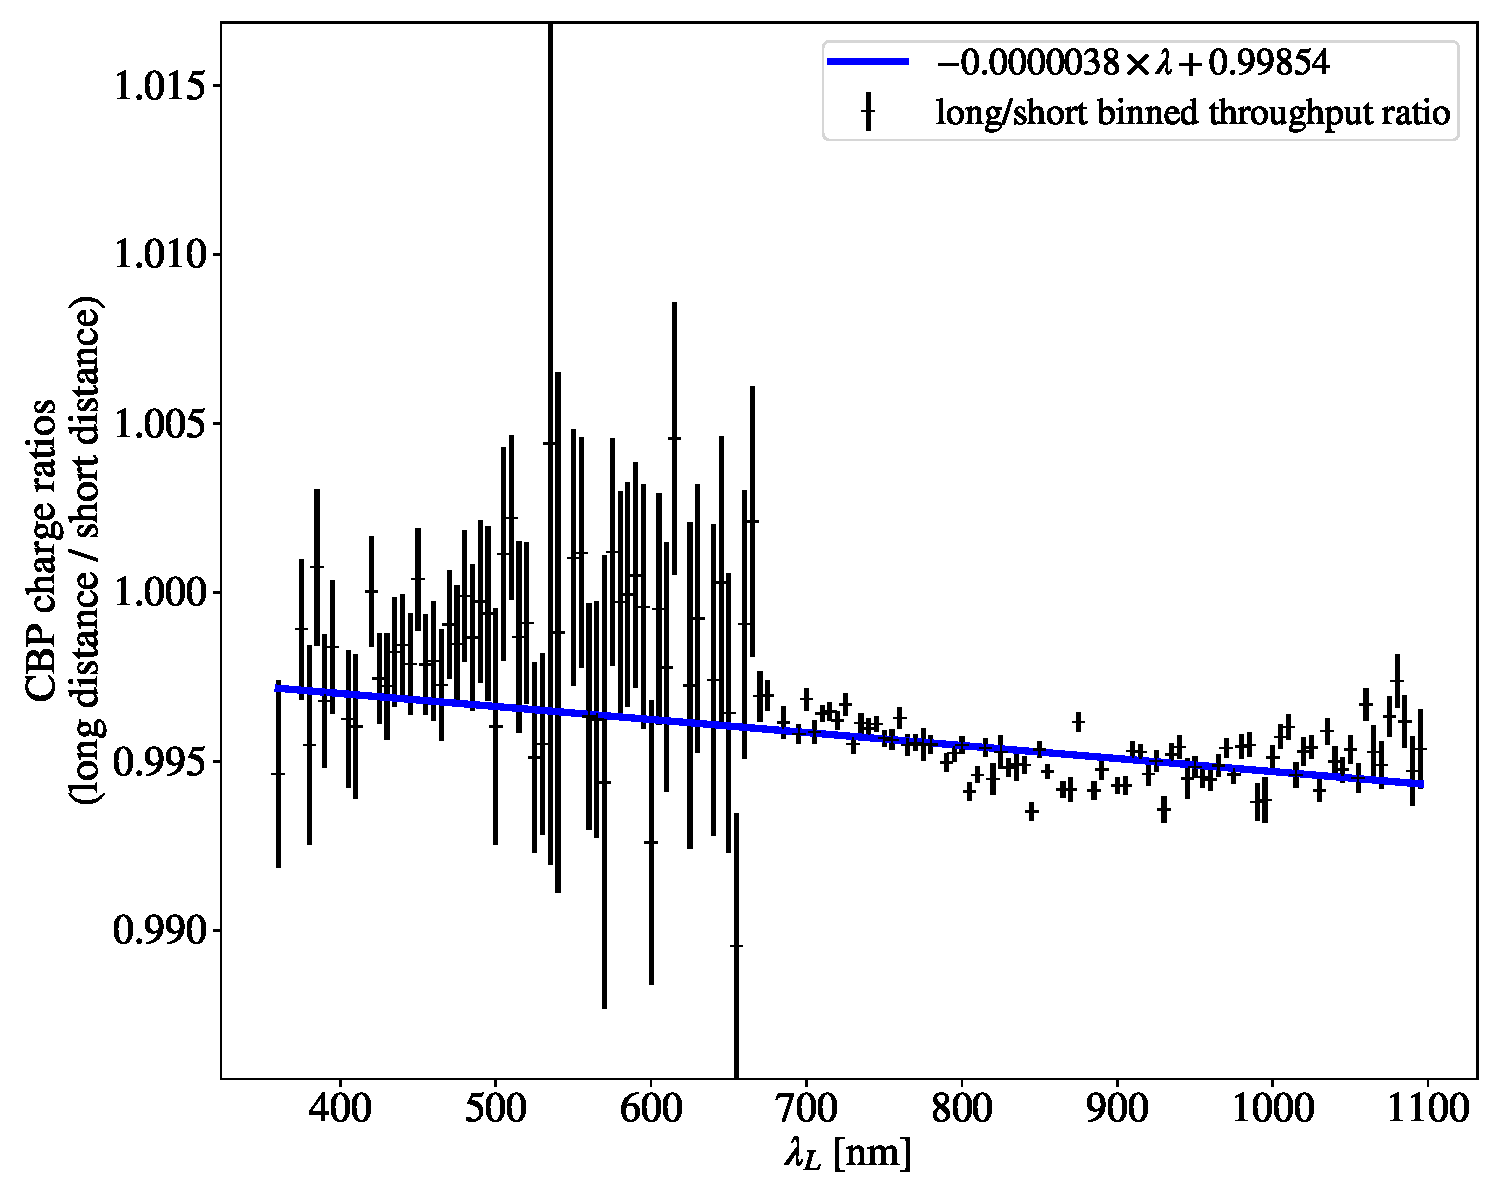
\includegraphics[width=\columnwidth]{fig/sc_distance.pdf}
    \caption{Ratios of the CBP charge ratio for two different distances to the solar cell as a function of $\lambda_L$ coming from the 2022/03/08 solar cell run. The long-distance is \SI{16}{\cm} larger than the short distance. Black points are the binned ratio for each $\lambda_L$, and the blue line is a fit whose equation is in legend.}
    \label{fig:sc_distance}
\end{figure}

\subsubsection{Solar cell QE variations with angle and temperature}

\todo{Do we write here the results ?}


\subsubsection{Repeatability}

Finally, we measured three times the value of the CBP response during our measurement campaign. For run $i$, we computed the CBP charge ratio $r_{\rm CBP}^{\mathrm{run}\ i}$, applying dark subtraction and laser contamination correction, binned in \SI{1}{\nano\meter} intervals in $\lambda_L$. Then, we computed the mean CBP response $\overline{r_{\rm CBP}}$ as the mean of the three different runs. We observed $\approx 1$\,permil differences between the three CBP charge ratios and $\overline{r_{\rm CBP}}$ (Figure~\ref{fig:SCrepeatability}), depending slightly with wavelength.


To assess the value of systematic uncertainties on the CBP response due to its stability, we take the maximum absolute distance of the binned ratio to unity in four different ranges of wavelengths (segments the farther from 1 in the bottom plot of Figure~\ref{fig:SCrepeatability}). The strongest systematics comes from the scattered light.

%cbp_paper_plots.ipynb
\begin{figure}[h]
    \centering
    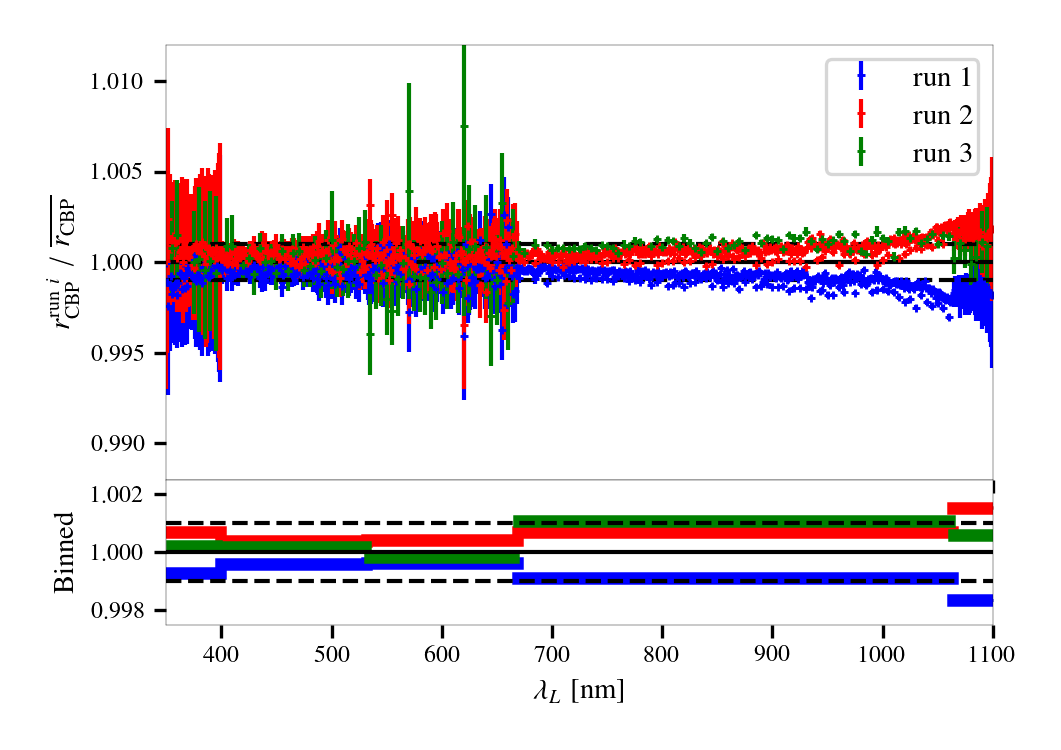
\includegraphics[width=\columnwidth]{fig/sc_runi_ratios.png}
    \caption{Ratios of the CBP charge ratio $r_{\rm CBP}^{\mathrm{run}\ i}\;/\;\overline{r_{\rm CBP}}$ for three different runs as a function of $\lambda_L$. Black dashed lines encompass the per-mil precision region. Top: ratios for each $\lambda_L$. Bottom: binned ratio for four different wavelength ranges.}
    \label{fig:SCrepeatability}
\end{figure}

\subsubsection{Summary}\label{sec:cbp_summary}

In summary, we defined the calibrated amount of charges in the solar cell as:
\begin{equation}
\Qsolarcal \equiv \Qsolarmes - \Qsolar^{\rm dark} - \Qsolar^{532} - \Qsolar^{\lambda_{\rm comp}} - \Qsolar^{\rm fluo}
\end{equation}
and in the photodiode as:
\begin{equation}
\Qphotcal(\lambda_L) = \left\lbrace
\begin{array}{ll}
          \Qphotmes(\lambda_L) - \Qphot^{\mathrm{fluo}}(\lambda_L) &\ \text{if}\ \lambda_L < \SI{400}{\nano\meter} \\
         \Qphotmes(\lambda_L)(1 + \alpha(\lambda_L)) &\ \text{if}\ \lambda_L \in \left[532, 644\right]\mathrm{\,nm} \\
        \Qphotmes(\lambda_L)(1 + \beta(\lambda_L)) &\ \text{if}\ \lambda_L > \SI{1064}{\nano\meter} \\
        \Qphotmes(\lambda_L)&\ \text{elsewhere}
\end{array}\right. 
\end{equation}

All uncertainties from the evaluation of all these terms were propagated. The summary of the error budget on the CBP response is decomposed in Figure~\ref{fig:cbp_budget} as a function of laser wavelength $\lambda_L$. Systematics coming from the wavelength calibration are not represented. Indeed, as the CBP response varies slowly with wavelength, it is negligible compared to others.  In the visible range, scattered light systematics dominates. In the far infrared, the subtraction of the $\lambda_{\mathrm{comp}}$ photons is the main systematic uncertainty, while in the UV range fluorescence correction systematic dominates.

%cbp_paper_plots.ipynb
\begin{figure}[h]
    \centering
    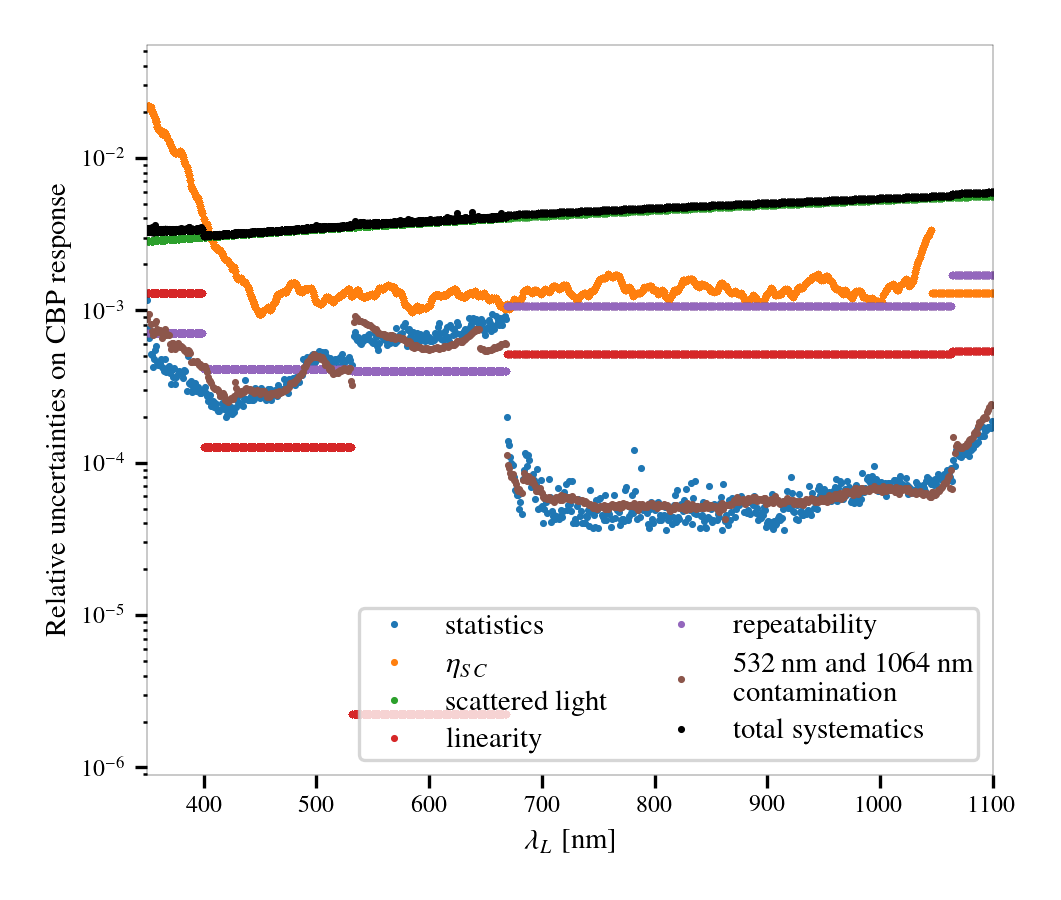
\includegraphics[width=\columnwidth]{fig/cbp_error_budget.png}
    \caption{Total error budget for CBP response.}
    \label{fig:cbp_budget}
\end{figure}

\subsection{CBP response}

The final CBP response in output photons per Coulomb unit in the photodiode is
\begin{equation}
    \Rcbp(\lambda_c) = \frac{\Qsolarcal(\lambda_c)}{\Qphotcal(\lambda_c) \times \epsilon_{\mathrm{solar}}(\lambda_c) \times e}.
    \label{eq:rcbp2}
\end{equation} 
It can be computed for each laser burst. We averaged the values to increase the signal-to-noise ratio and get the red smooth curve presented in Figure~\ref{fig:cbp_response}:
\begin{equation}
    \overline{\Rcbp(\hat{\lambda}_c)} = \left\langle\frac{\Qsolarcal(\lambda_c)}{\Qphotcal(\lambda_c) \times \epsilon_{\mathrm{solar}}(\lambda_c) \times e}\right\rangle_{\lambda_c\in [\lambda,\lambda+\delta \lambda]}.
    \label{eq:rcbp3}
\end{equation} 
The average is performed on every burst of the three runs, with a $5\sigma$ clipping, and $\hat{\lambda}_c$ is the mean calibrated wavelength in a $\delta \lambda = \SI{1}{\nano\meter}$ bin. All uncertainties are combined in quadrature (Figure~\ref{fig:cbp_response} bottom). The total uncertainty is between 3 and $5\,$permil \todo{Check this statement at the end of the analysis as only the chromatic part is important.} in the visible range, due to scattered light systematic, and slightly higher in the UV and IR ranges.



%cbp_paper_plots.ipynb
\begin{figure}[h]
    \centering
    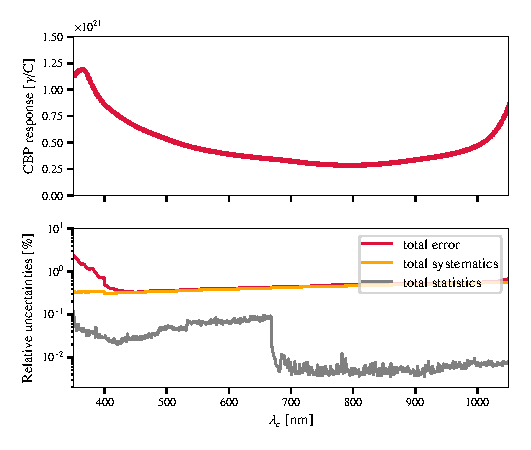
\includegraphics[width=\columnwidth]{fig/cbp_response.pdf}
    \caption{Top: CBP response $\overline{\Rcbp(\hat{\lambda}_c)}$ obtained with the \bpinhole and $\delta \lambda = \SI{1}{\nano\meter}$. Bottom: relative uncertainties.}
    \label{fig:cbp_response}
\end{figure}